\documentclass[titlepage]{article}

\usepackage[letterpaper,margin=1in,footskip=0.25in]{geometry}
\usepackage[hidelinks]{hyperref}
\usepackage{fancyhdr}
\usepackage{csquotes}
\usepackage{amsmath}
\usepackage{amssymb}
\usepackage{tikz}
\usepackage[nottoc,notlof,notlot]{tocbibind}
\usepackage{subcaption}

\MakeOuterQuote{"}

\newcounter{theorem}
\newcommand{\newtrm}[1]{\refstepcounter{theorem}\label{#1}Theorem \thetheorem: }

\numberwithin{figure}{section}
\numberwithin{equation}{section}
\numberwithin{theorem}{section}

\usetikzlibrary{calc,positioning,through,matrix,decorations.markings,shapes.geometric}

\newcommand{\R}{\mathbb{R}}
\newcommand{\C}{\mathbb{C}}
\newcommand{\F}{\mathbb{F}}
\newcommand{\dq}[4][]{``#2"#1 \cite[#4]{#3}.}

\newcommand{\Blu}{$\color{blue!30}B$}
\newcommand{\Red}{$\color{red!30}R$}
\newcommand{\Gre}{$\color{green!30}G$}
\newcommand{\Whi}{$W$}

\newcommand{\V}{\mathcal{V}}
\newcommand{\E}{\mathcal{E}}
\newcommand{\G}{\mathcal{G}}
\newcommand{\K}{\mathcal{K}}
\newcommand{\Li}{\mathcal{L}}

\newcommand{\T}{\text{T}}

\renewcommand{\labelitemiii}{\scriptsize$\blacksquare$}

\title{GIEP Notes}
\author{Steven Labalme}
\date{\today}

\begin{document}




\pagenumbering{gobble}
\maketitle



\pagenumbering{roman}
\tableofcontents
\listoffigures
\newpage



\pagenumbering{arabic}
\pagestyle{fancy}
\fancyhf{}
\rfoot{Labalme \thepage}
\renewcommand{\headrulewidth}{0pt}
\section{Vector Spaces}
\subsection{$\R^n$ and $\C^n$}
From \cite{bib:Axler}.
\begin{itemize}
    \item Assumed familiarity with the set $\R$ of real numbers.
    \item \textbf{Complex number}: An ordered pair $(a,b)$, where $a,b\in\R$, but we will write this as $a+bi$.
    \begin{itemize}
        \item The set of all complex number is denoted by $\C$:
        \begin{equation*}
            \C = \{a+bi:a,b\in\R\}^[\footnote{The complex numbers equal the set of numbers $a+bi$ such that $a$ and $b$ are elements of the real numbers.}^]
        \end{equation*}
        \item Definitions of \textbf{addition} and \textbf{multiplication} on $\C$ are given, but I know these.
    \end{itemize}
    \item Properties of complex arithmetic:
    \begin{itemize}
        \item \textbf{Commutativity}: $\alpha+\beta=\beta+\alpha$ and $\alpha\beta=\beta\alpha$ for all $\alpha,\beta\in\C$.
        \item \textbf{Associativity}: $(\alpha+\beta)+\lambda=\alpha+(\beta+\lambda)$ and $(\alpha\beta)\lambda=\alpha(\beta\lambda)$ for all $\alpha,\beta,\lambda\in\C$.
        \item \textbf{Identities}: $\lambda+0=\lambda$ and $\lambda 1=\lambda$ for all $\lambda\in\C$.
        \item \textbf{Additive inverse}: For every $\alpha\in\C$, there exists a unique $\beta\in\C$ such that $\alpha+\beta=0$.
        \item \textbf{Multiplicative inverse}: For every $\alpha\in\C$ with $\alpha\neq0$, there exists a unique $\beta\in\C$ such that $\alpha\beta=1$.
        \item \textbf{Distributive property}: $\lambda(\alpha+\beta)=\lambda\alpha+\lambda\beta$ for all $\lambda,\alpha,\beta\in\C$.
    \end{itemize}
    \item \dq{The properties above are proved using the familiar properties of real numbers and the definitions of complex addition and multiplication}{bib:Axler}{3}
    \item $\F$ stands for $\R$ or $\C$.
    \begin{itemize}
        \item Any theorem proved with $\F$ holds when $\F$ is replaced with $\R$ and when $\F$ is replaced with $\C$.
    \end{itemize}
    \item \textbf{Scalar}: A number or magnitude. This word is commonly used to differentiate a quantity from a \textbf{vector} quantity.
    \item Subtraction and division are defined.
    \item Properties of exponents are defined.
    \item The set $\R^2$, which can be conceived as a plane, is the set of all \textbf{ordered pairs} of real numbers:
    \begin{equation*}
        \R^2 = \left\{ (x,y):x,y\in\R \right\}
    \end{equation*}
    \item The set $\R^3$, which can be conceived as ordinary space, is the set of all \textbf{ordered triples} of real numbers:
    \begin{equation*}
        \R^3 = \left\{ (x,y,z):x,y,z\in\R \right\}
    \end{equation*}
    \item \dq
        {Suppose $n$ is a nonnegative integer. A \textbf{list} of \textbf{length} $n$ is an ordered collection of $n$ elements (which might be numbers, other lists, or more abstract entities) separated by commas and surrounded by parentheses. A list of length $n$ looks like this:
        \begin{equation*}
            (x_1,\dots,x_n)
        \end{equation*}
        Two lists are equal if and only if they have the same length and the same elements in the same order}
    {bib:Axler}{5}
    \item \textbf{Ordered pair}: A list of length 2.
    \item \textbf{Ordered triple}: A list of length 3.
    \item \textbf{$n$-tuple}: A list of length $n$.
    \item Although lists are sometimes discussed without specifying their length, a list must, by definition, have a finite length, i.e. $(x_1,x_2,\dots)$ is not a list.
    \item A list of length 0 looks like this: $()$.
    \begin{itemize}
        \item Such an object is defined to avoid trivial exceptions to theorems.
    \end{itemize}
    \item Lists vs. \textbf{sets}: In lists, order matters and repetitions have meaning. In sets, order and repetitions are irrelevant.
    \item \dq
        {$\mathbf{\F^n}$ is the set of all lists of length $n$ of elements of $\F$:
        \begin{equation*}
            \F^n = \left\{ (x_1,\dots,x_n):x_j\in\F\text{ for }j=1,\dots,n)\right\}
        \end{equation*}
        For $(x_1,\dots,x_n)\in\F^n$ and $j\in\left\{ 1,\dots,n \right\}$, we say that $x_j$ is the $j^\text{th}$ \textbf{coordinate} of $(x_1,\dots,x_n)$}
    {bib:Axler}{6}
    \item For help in conceiving higher dimensional spaces, consider reading \emph{Flatland: A Romance of Many Dimensions} by Edwin A. Abbot. This is an amusing account of how $\R^3$ would be perceived by creatures living in $\R^2$.
    \item \textbf{Addition} (in $\F^n$): Add corresponding coordinates:
    \begin{equation*}
        (x_1,\dots,x_n)+(y_1,\dots,y_n)=(x_1+y_1,\dots,x_n+y_n)
    \end{equation*}
    \item For a simpler notation, use a single letter to denote a list of $n$ numbers.
    \begin{itemize}
        \item \textbf{Commutativity} (of addition in $\F^n$): If $x,y\in\F^n$, then $x+y=y+x$.
        \item However, the proof still requires the more formal, cumbersome list notation$^[$\footnote{Note that $\blacksquare$ means "end of the proof."}$^]$.
    \end{itemize}
    \item $\mathbf{0}$: The list of length $n$ whose coordinates are all 0:
    \begin{equation*}
        0=(0,\dots,0)
    \end{equation*}
    \begin{itemize}
        \item Although the ambiguity in the use of "0" on the left vs. right side of the equation may seem confusing, context can always differentiate between which definition is needed.
    \end{itemize}
    \item A picture can help visualize $\R^2$ because $\R^2$ can be sketched on 2-dimensional surfaces such as paper.
    \begin{figure}[h]
        \centering
        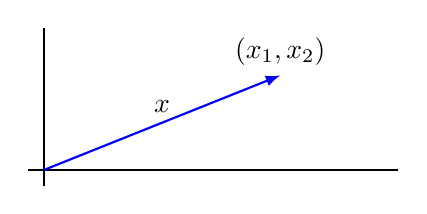
\begin{tikzpicture}[every node/.append style={above,black}]
            \draw (-0.2,0) -- (4.5,0);
            \draw (0,-0.2) -- (0,1.8);
            \draw[blue,thick,-latex] (0,0) -- node{$x$} (3,1.2) node{$(x_1,x_2)$};
        \end{tikzpicture}
        \caption{$x\in\R^2$ can be conceived as a point or a vector.}
        \label{fig:axesvector}
    \end{figure}
    \begin{itemize}
        \item A typical element of $\R^2$ is a point $x=(x_1,x_2)$.
        \item However, points are generally though of as an arrow starting at the origin and ending at $x$, as shown below.
        \item When thought of as an arrow, $x$ is called a \textbf{vector}.
        \item When translated without varying length or direction, it is still the same vector.
        \item Remember that these pictures are aids --- although we cannot visualize higher dimensional vector spaces, the algebraic elements are as rigorously defined as those of $\R^2$.
    \end{itemize}
    \item Addition has a simple geometric interpretation in $\R^2$.
    \item If we want to add $x+y$, slide $y$ so that its initial point coincides with the terminal point of $x$. The sum is the vector from the tail of $x$ to the head of $y$.
    \begin{figure}[h]
        \centering
        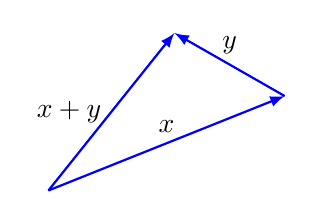
\begin{tikzpicture}[
            every node/.append style={black},
            every path/.append style={blue,thick,-latex}
        ]
            \coordinate (a) at (0,0);
            \coordinate (b) at (3,1.2);
            \coordinate (c) at (1.6,2);

            \draw (a) -- node[above]{$x$}   (b);
            \draw (b) -- node[above]{$y$}   (c);
            \draw (a) -- node[left] {$x+y$} (c);
        \end{tikzpicture}
        \caption{Vector addition.}
        \label{fig:addvectors}
    \end{figure}
    \item \dq
        {For $x\in\F^n$, the \textbf{additive inverse} of $x$, denoted $-x$, is the vector $-x\in\F^n$ such that
        \begin{equation*}
            x+(-x)=0
        \end{equation*}
        In other words, if $x=\left( x_1,\dots,x_n \right)$, then $-x=\left( -x_1,\dots,-x_n \right)$}
    {bib:Axler}{9}
    \begin{figure}[h]
        \centering
        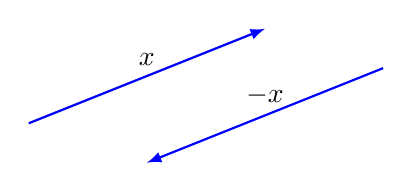
\begin{tikzpicture}[
            every node/.append style={above,black},
            every path/.append style={blue,thick,-latex}
        ]
            \coordinate (a) at (0,0);
            \coordinate (b) at (3,1.2);

            \draw (a) -- node{$x$} (b);
            \draw ($(b)+(1.5,-0.5)$) -- node{$-x$} ($(a)+(1.5,-0.5)$);
        \end{tikzpicture}
        \caption{A vector and its additive inverse.}
        \label{fig:invvectors}
    \end{figure}
    \begin{itemize}
        \item For $x\in\R^2$, $-x$ is the vector parallel to $x$ with the same length but in the opposite direction.
    \end{itemize}
    \item \textbf{Product (scalar multiplication)}: When multiplying $\lambda\in\F$ and $x\in\F^n$, multiply each coordinate of $x$ by $\lambda$:
    \begin{equation*}
        \lambda\left( x_1,\dots,x_n \right)=\left( \lambda x_1,\dots,\lambda x_n \right)
    \end{equation*}
    \begin{figure}[h]
        \centering
        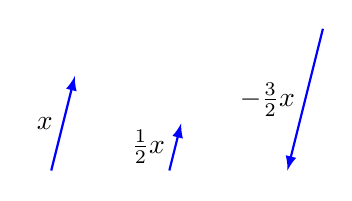
\begin{tikzpicture}[
            every node/.append style={left,black},
            every path/.append style={blue,thick,-latex}
        ]
            \coordinate (a) at (0,0);
            \coordinate (b) at (0.3,1.2);

            \draw (a) -- node{$x$} (b);
            \draw ($(a)+(1.5,0)$) -- node{$\tfrac{1}{2}x$} ($(b)+(1.35,-0.6)$);
            \draw (3.45,1.8) -- node{$-\tfrac{3}{2}x$} ($(a)+(3,0)$);
        \end{tikzpicture}
        \caption{Scalar multiplication.}
        \label{fig:multvector}
    \end{figure}
    \item \textbf{Field}: A \dq[ of complex arithmetic (see earlier in this section)]{set containing at least two distinct elements called 0 and 1, along with operations of addition and multiplication satisfying all the properties}{bib:Axler}{10}
\end{itemize}


\subsection{Definition of Vector Space}
\begin{itemize}
    \item \textbf{Addition (on a set \emph{V})}: \dq{A function that assigns an element $u+v\in V$ to each pair of elements $u,v\in V$}{bib:Axler}{12}
    \item \textbf{Scalar multiplication (on a set \emph{V})}: \dq{A function that assigns an element $\lambda v\in V$ to each $\lambda\in\F$ and each $v\in V$}{bib:Axler}{12}
    \item \textbf{Vector space}: \dq
        {A set $V$ along with an addition and a scalar multiplication on V such that the following properties hold:}
    {bib:Axler}{12}
    \begin{description}
        \item[commutativity] \hfill \\ $u+v=v+u$ for all $u,v\in V$
        \item[associativity] \hfill \\ $(u+v)+w=u+(v+w)$ and $(ab)v=a(bv)$ for all $u,v,w\in V$ and all $a,b\in \F$
        \item[additive identity] \hfill \\ There exists an element $0\in V$ such that $v+0=v$ for all $v\in V$
        \item[additive inverse] \hfill \\ For every $v\in V$, there exists $w\in V$ such that $v+w=0$
        \item[multiplicative identity] \hfill \\ $1v=v$ for all $v\in V$
        \item[distributive properties] \hfill \\ $a(u+v)=au+av$ and $(a+b)v=av+bv$ for all $a,b\in\F$ and all $u,v\in V$
    \end{description}
    \item To be more precise, $V$ depends on $\F$, so sometimes we say $V$ is a \textbf{vector space over $\F$}.
    \begin{itemize}
        \item For example, $\R^n$ is only a vector space over $\R$, not $\C$.
    \end{itemize}
    \item \textbf{Real vector space}: A vector space over $\R$.
    \item \textbf{Complex vector space}: A vector space over $\C$.
    \item $\F^\infty$ is a vector space.
    \item $\F^S$ denotes the set of functions from $S$ to $\F$.
    \begin{itemize}
        \item For example, $\R^{\left[ 0,1 \right]}$ is the \dq{set of real-valued functions on the interval $\left[ 0,1 \right]$}{bib:Axler}{14}
        \item You can think of $\F^n$ as $\F^{\left\{ 1,2,\dots,n\right\}}$.
    \end{itemize}
    \item Elementary properties of vector spaces:
    \begin{itemize}    
        \item A vector space has a unique additive identity.
        \begin{itemize}
            \item Suppose $0$ and $0'$ are both additive identities in V. Then
            \begin{equation*}
                0' = 0'+0 = 0+0' = 0
            \end{equation*}
            The first equality holds due to $0$ being an additive identity. The second holds due to commutativity. The third holds due to $0'$ being an additive identity. Thus, $0=0'$, and $V$ has only one additive identity.
        \end{itemize}
        \item Each element $v\in V$ has a unique additive inverse.
        \begin{itemize}
            \item Same idea:
            \begin{equation*}
                w = w+0 = w+(v+w') = (w+v)+w' = 0+w' = w'
            \end{equation*}
        \end{itemize}
        \item $0v=0\ \forall\ v\in V$, where $0$ on the left side is a scalar and $0$ on the right side is a vector (the additive identity of $V$).
        \begin{itemize}
            \item Since this property asserts something about both scalar multiplication and the additive identity, the distributive property (the only part of the definition of a vector space that connects scalar multiplication and vector addition) must be used in the proof.
            \begin{align*}
                0v &= (0+0)v\\
                0v &= 0v+0v\\
                0v-0v &= 0v+0v-0v\\
                0 &= 0v
            \end{align*}
        \end{itemize}
        \item $a0=0\ \forall\ a\in\F$, where $0$ is a vector.
        \begin{itemize}
            \item Same as above.
        \end{itemize}
        \item $(-1)v=-v\ \forall\ v\in V$, where $-1$ is a scalar and $-v$ is the additive inverse of $v$.
        \begin{equation*}
            v+(-1)v=1v+(-1)v=(1+(-1))v=0v=0
        \end{equation*}
    \end{itemize}
\end{itemize}


\subsection{Subspaces}
\begin{itemize}
    \item \textbf{Subspace}: A subset $U$ of $V$ that is a vector space under the same definition of addition and scalar multiplication as on $V$, e.g., satisfies the following three conditions.
    \begin{description}
        \item[additive identity] \hfill \\ $0\in U$
        \item[closed under addition] \hfill \\ $u,w\in U$ implies $u+w\in U$
        \item[closed under scalar multiplication] \hfill \\ $a\in\F$ and $u\in U$ implies $au\in U$  
    \end{description}
    \item The other conditions can be derived from the above 3.
    \item When we look at subspaces within the differentiable functions, the logical foundation of calculus appears.
    \item The subspaces of $\R^2$ are $\{0\}$, $\R^2$, and any straight line through the origin.
    \item The subspaces of $\R^3$ are $\{0\}$, $\R^3$, any straight line through the origin, and any flat plane through the origin.
    \item \textbf{Sum of subsets}: If $U_1,\dots,U_n$ are subsets of $V$, their \textbf{sum} (denoted $U_1+\cdots+U_n$) is the set of all possible sums of elements of $U_1,\dots,U_n$:
    \begin{equation*}
        U_1+\cdots+U_m = \left\{ u_1+\cdots+u_m:u_1\in U_1,\dots,u_m\in U_m \right\}
    \end{equation*}
    \item The sum of subspaces is the smallest containing subspace.
    \begin{itemize}
        \item Clearly, the sum of subspaces is a subspace (satisfies 3 tenets).
        \item The sum of subspaces contains every original element ($u_1$ plus the $0$ from $u_2$, etc.). Any subspace containing all of these elements must contain every finite sum of them (by definition). Thus, no smaller subspace can be created than that of the sum of every element.
    \end{itemize}
    \item \textbf{Direct sum}: A sum of subspaces where each element of $U_1+\cdots+U_m$ can be written in only one way as a sum $u_1+\cdots+u_m$.
    \begin{itemize}
        \item $U_1\oplus\dots\oplus U_m$ denotes $U_1+\cdots+U_m$ if $U_1+\cdots+U_m$ is a direct sum.
    \end{itemize}
    \item A sum of subspaces is a direct sum if and only if the only way to write $0$ as a sum of elements is by summing the $0$ of each subset.
    \item A sum of subspaces $U$ and $W$ is a direct sum if and only if $U\cap W=\{0\}$.
\end{itemize}
\newpage



\section{Graphs}
\subsection{A Gentle Introduction}
From \cite{bib:graph}.
\begin{itemize}
    \item Begins with the K\"{o}nigsberg Bridge Problem and Euler's solution by reducing the land masses to a mathematical \textbf{graph}.
    \item Finding an abstract mathematical model of a concrete problem requires ingenuity and experience. \dq{The primary aim of this chapter is to provide the reader with some of this experience by presenting several real-world problems and showing how they can be formulated in mathematical terms}{bib:graph}{277-78}
    \item Considers the Three Houses--Three Utilities Problem.
    \item Deeply considers Instant Insanity (stack four cubes, each with one of four colors on each face, in such a way that every color is represented on every side of the column):
    \begin{figure}[h!]
        \centering
        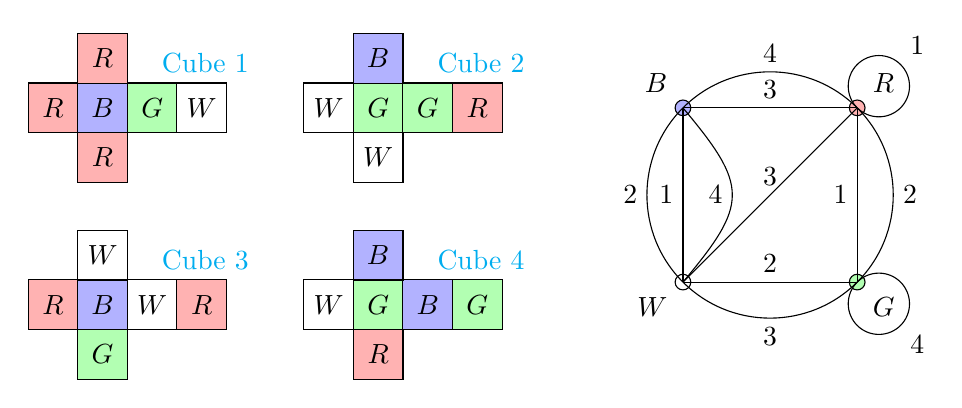
\begin{tikzpicture}
            \colorlet{rex}{red!30}
            \colorlet{blx}{blue!30}
            \colorlet{grx}{green!30}
    
    
            \begin{scope}[
                node distance=-0.42pt,
                every node/.style={draw,minimum size=6.3mm}
            ]
                \node (a1) [fill=rex]             {$R$};
                \node (b1) [right=of a1,fill=blx] {$B$};
                \node (c1) [right=of b1,fill=grx] {$G$};
                \node (d1) [right=of c1]          {$W$};
                \node (e1) [above=of b1,fill=rex] {$R$};
                \node (f1) [below=of b1,fill=rex] {$R$};
            \end{scope}
            \node [above right,cyan] at (c1.90) {Cube 1};
    
            \begin{scope}[
                node distance=-0.42pt,
                every node/.style={draw,minimum size=6.3mm},
                xshift=35mm
            ]
                \node (a2)                        {$W$};
                \node (b2) [right=of a2,fill=grx] {$G$};
                \node (c2) [right=of b2,fill=grx] {$G$};
                \node (d2) [right=of c2,fill=rex] {$R$};
                \node (e2) [above=of b2,fill=blx] {$B$};
                \node (f2) [below=of b2]          {$W$};
            \end{scope}
            \node [above right,cyan] at (c2.90) {Cube 2};
    
            \begin{scope}[
                node distance=-0.42pt,
                every node/.style={draw,minimum size=6.3mm},
                yshift=-25mm
            ]
                \node (a3) [fill=rex]             {$R$};
                \node (b3) [right=of a3,fill=blx] {$B$};
                \node (c3) [right=of b3]          {$W$};
                \node (d3) [right=of c3,fill=rex] {$R$};
                \node (e3) [above=of b3]          {$W$};
                \node (f3) [below=of b3,fill=grx] {$G$};
            \end{scope}
            \node [above right,cyan] at (c3.90) {Cube 3};
    
            \begin{scope}[
                node distance=-0.42pt,
                every node/.style={draw,minimum size=6.3mm},
                xshift=35mm,yshift=-25mm
            ]
                \node (a4)                        {$W$};
                \node (b4) [right=of a4,fill=grx] {$G$};
                \node (c4) [right=of b4,fill=blx] {$B$};
                \node (d4) [right=of c4,fill=grx] {$G$};
                \node (e4) [above=of b4,fill=blx] {$B$};
                \node (f4) [below=of b4,fill=rex] {$R$};
            \end{scope}
            \node [above right,cyan] at (c4.90) {Cube 4};
    
    
            \begin{scope}[
                node distance=2cm,
                every node/.style={circle,draw,inner sep=2pt},
                xshift=8cm
            ]
                \node (B) [fill=blx]            {};
                \node (R) [right=of B,fill=rex] {};
                \node (W) [below=of B]          {};
                \node (G) [right=of W,fill=grx] {};
            \end{scope}
            \node [above left]  at (B.135)  {$B$};
            \node [above right] at (R.45)   {$R$};
            \node [below left]  at (W.-135) {$W$};
            \node [below right] at (G.-45)  {$G$};
            \draw (B.center) --                             node[above]{3} (R.center);
            \draw (B.center) --                             node[left] {1} (W.center);
            \draw (R.center) --                             node[left] {1} (G.center);
            \draw (W.center) --                             node[above]{2} (G.center);
            \draw (B.center) to[bend left=45]               node[above]{4} (R.center);
            \draw (B.center) to[bend right=45]              node[left] {2} (W.center);
            \draw (R.center) to[bend left=45]               node[right]{2} (G.center);
            \draw (W.center) to[bend right=45]              node[below]{3} (G.center);
            \draw (W.center) --                             node[above]{3} (R.center);
            \draw (B.center) to[bend left=40,distance=13mm] node[left] {4} (W.center);
            \node (Rcirc) [draw,circle through={(R.center)}] at ($(R.45)+(0.2,0.2)$)   {};
            \node (Gcirc) [draw,circle through={(G.center)}] at ($(G.-45)+(0.2,-0.2)$) {};
            \node at (Rcirc.45) [above right] {1};
            \node at (Gcirc.-45) [below right] {4};
        \end{tikzpicture}
        \caption{Four colored cubes and a graphical representation.}
        \label{fig:cubesgraph}
    \end{figure}
    \item Each vertex in Figure \ref{fig:cubesgraph} represents one of the colors. Each edge connects a color on one face of a cube to the color on the opposite face (the cube to which this relationship pertains is identified by the number along the edge).
    \begin{itemize}
        \item For example, \Blu\ is connected to \Red\ by a line with $3$ above it because on \textcolor{cyan}{Cube 3}, the blue face and the red face are on opposite sides of the cube.
    \end{itemize}
    \item Let's take a look at a possible stack and see what we can learn from it and its \textbf{subgraph} (see Figure \ref{fig:stack1graph}).
    \begin{figure}[h!]
        \centering
        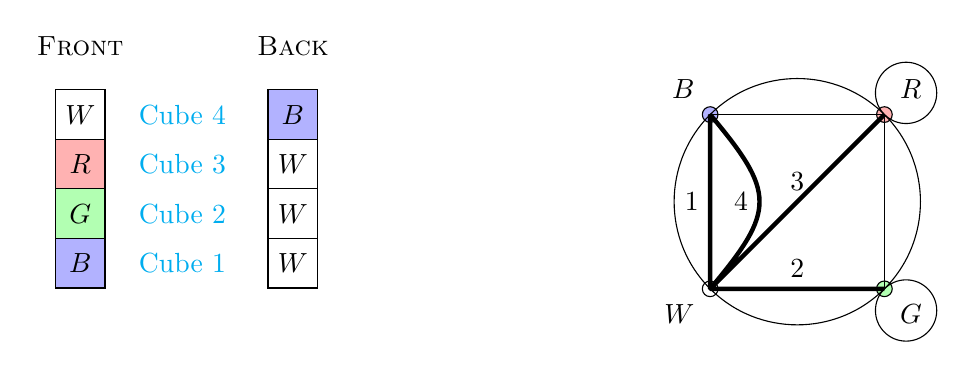
\begin{tikzpicture}[
            node distance=3mm
        ]
            \colorlet{rex}{red!30}
            \colorlet{blx}{blue!30}
            \colorlet{grx}{green!30}
    
    
            \begin{scope}[
                node distance=-0.42pt,
                every node/.style={draw,minimum size=6.3mm}
            ]
                \node (a1)                        {$W$};
                \node (b1) [below=of a1,fill=rex] {$R$};
                \node (c1) [below=of b1,fill=grx] {$G$};
                \node (d1) [below=of c1,fill=blx] {$B$};
            \end{scope}
            \node [above=of a1,font=\scshape] {Front};
            \node [right=of a1,cyan] {Cube 4};
            \node [right=of b1,cyan] {Cube 3};
            \node [right=of c1,cyan] {Cube 2};
            \node [right=of d1,cyan] {Cube 1};
    
            \begin{scope}[
                node distance=-0.42pt,
                every node/.style={draw,minimum size=6.3mm},
                xshift=27mm
            ]
                \node (a2) [fill=blx]    {$B$};
                \node (b2) [below=of a2] {$W$};
                \node (c2) [below=of b2] {$W$};
                \node (d2) [below=of c2] {$W$};
            \end{scope}
            \node [above=of a2,font=\scshape] {Back};
    
    
            \begin{scope}[
                node distance=2cm,
                every node/.style={circle,draw,inner sep=2pt},
                xshift=8cm
            ]
                \node (B) [fill=blx]            {};
                \node (R) [right=of B,fill=rex] {};
                \node (W) [below=of B]          {};
                \node (G) [right=of W,fill=grx] {};
            \end{scope}
            \node [above left]  at (B.135)  {$B$};
            \node [above right] at (R.45)   {$R$};
            \node [below left]  at (W.-135) {$W$};
            \node [below right] at (G.-45)  {$G$};
            \draw               (B.center) --                                            (R.center);
            \draw               (R.center) --                                            (G.center);
            \draw               (B.center) to[bend left=45]                              (R.center);
            \draw               (B.center) to[bend right=45]                             (W.center);
            \draw               (R.center) to[bend left=45]                              (G.center);
            \draw               (W.center) to[bend right=45]                             (G.center);
            \draw [ultra thick,line join=bevel] (R.center) -- node[above]{3} (W.center) to[bend right=40,distance=13mm] node[left] {4} (B.center) -- node[left] {1} (W.center) -- node[above]{2} (G.center);
            \node (Rcirc) [draw,circle through={(R.center)}] at ($(R.45)+(0.2,0.2)$)   {};
            \node (Gcirc) [draw,circle through={(G.center)}] at ($(G.-45)+(0.2,-0.2)$) {};
        \end{tikzpicture}
        \caption{A possible stacking and graph.}
        \label{fig:stack1graph}
    \end{figure}
    \item The reason this stack fails to provide a correct column, front and back, is because too many edges touch white and not enough touch red or green.
    \item Also note that this subgraph represents a feasible stack because each cube is represented once (each number appears once in the subgraph).
    \item Therefore, we can conjecture conditions of the subgraph that will lead to a stack that is solved front-to-back, namely:
    \begin{itemize}
        \item The subgraph will contain all four vertices.
        \item The subgraph will consist of four edges, one from each cube.
        \item The subgraph will have exactly two edges meeting at each vertex.
    \end{itemize}
    \item Following these strictures, several graphs can be easily drawn. One such graph is shown in Figure \ref{fig:stack2graph} in correspondence with two columns (this is also the solution to Pause 1).
    \begin{figure}[h!]
        \centering
        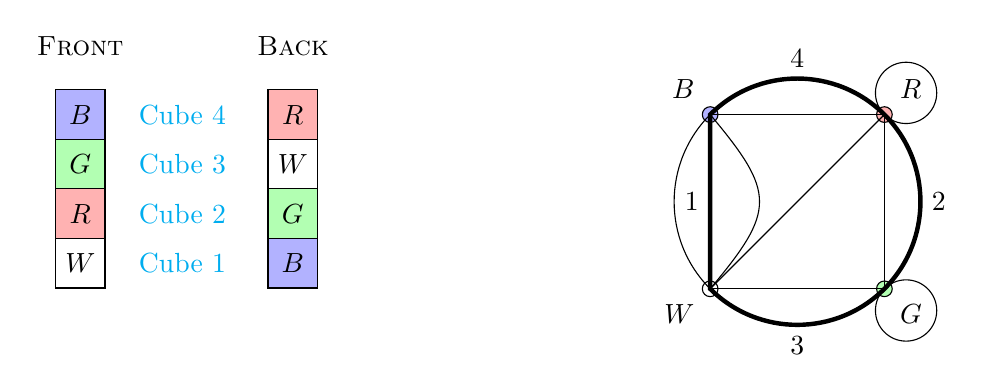
\begin{tikzpicture}[
            node distance=3mm
        ]
            \colorlet{rex}{red!30}
            \colorlet{blx}{blue!30}
            \colorlet{grx}{green!30}
    
    
            \begin{scope}[
                node distance=-0.42pt,
                every node/.style={draw,minimum size=6.3mm}
            ]
                \node (a1) [fill=blx]             {$B$};
                \node (b1) [below=of a1,fill=grx] {$G$};
                \node (c1) [below=of b1,fill=rex] {$R$};
                \node (d1) [below=of c1]          {$W$};
            \end{scope}
            \node [above=of a1,font=\scshape] {Front};
            \node [right=of a1,cyan] {Cube 4};
            \node [right=of b1,cyan] {Cube 3};
            \node [right=of c1,cyan] {Cube 2};
            \node [right=of d1,cyan] {Cube 1};
    
            \begin{scope}[
                node distance=-0.42pt,
                every node/.style={draw,minimum size=6.3mm},
                xshift=27mm
            ]
                \node (a2) [fill=rex]             {$R$};
                \node (b2) [below=of a2]          {$W$};
                \node (c2) [below=of b2,fill=grx] {$G$};
                \node (d2) [below=of c2,fill=blx] {$B$};
            \end{scope}
            \node [above=of a2,font=\scshape] {Back};
    
    
            \begin{scope}[
                node distance=2cm,
                every node/.style={circle,draw,inner sep=2pt},
                xshift=8cm
            ]
                \node (B) [fill=blx]            {};
                \node (R) [right=of B,fill=rex] {};
                \node (W) [below=of B]          {};
                \node (G) [right=of W,fill=grx] {};
            \end{scope}
            \node [above left]  at (B.135)  {$B$};
            \node [above right] at (R.45)   {$R$};
            \node [below left]  at (W.-135) {$W$};
            \node [below right] at (G.-45)  {$G$};
            \draw               (B.center) --                                            (R.center);
            \draw               (R.center) --                                            (G.center);
            \draw               (W.center) --                                            (G.center);
            \draw               (B.center) to[bend right=45]                             (W.center);
            \draw               (W.center) --                                            (R.center);
            \draw               (B.center) to[bend left=40,distance=13mm]                (W.center);
            \draw [ultra thick] (B.center) -- node[left] {1} (W.center) to[bend right=45] node[below]{3} (G.center) to[bend right=45] node[right]{2} (R.center) to[bend right=45] node[above]{4} cycle;
            \node (Rcirc) [draw,circle through={(R.center)}] at ($(R.45)+(0.2,0.2)$)   {};
            \node (Gcirc) [draw,circle through={(G.center)}] at ($(G.-45)+(0.2,-0.2)$) {};
        \end{tikzpicture}
        \caption{A front-to-back-solved stacking and graph.}
        \label{fig:stack2graph}
    \end{figure}
    \item Getting the front and back correct is comparably easy to getting the sides correct when playing with the toy.
    \item Graphically, there must be a second subgraph that satisfies the above conditions and is \textbf{edge disjoint} from the first.
    \item \textbf{Edge disjoint} (subgraphs): Two subgraphs that share no edges between them.
    \item Figure \ref{fig:insanesolution} shows two edge disjoint subgraphs superimposed on the same graph.
    \begin{figure}[h!]
        \centering
        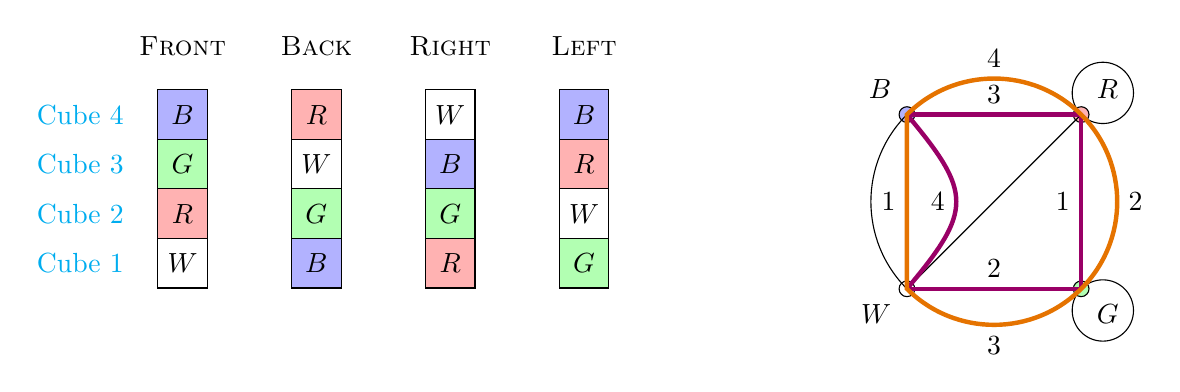
\begin{tikzpicture}[
            node distance=3mm
        ]
            \colorlet{rex}{red!30}
            \colorlet{blx}{blue!30}
            \colorlet{grx}{green!30}
            \colorlet{orx}{orange!90!black}
            \colorlet{pux}{red!60!blue}
    
    
            \begin{scope}[
                node distance=-0.42pt,
                every node/.style={draw,minimum size=6.3mm}
            ]
                \node (a1) at (1.8,0) [fill=blx]             {$B$};
                \node (b1) [below=of a1,fill=grx] {$G$};
                \node (c1) [below=of b1,fill=rex] {$R$};
                \node (d1) [below=of c1]          {$W$};
            \end{scope}
            \node [above=of a1,font=\scshape] {Front};
            \node [left=of a1,cyan] {Cube 4};
            \node [left=of b1,cyan] {Cube 3};
            \node [left=of c1,cyan] {Cube 2};
            \node [left=of d1,cyan] {Cube 1};
    
            \begin{scope}[
                node distance=-0.42pt,
                every node/.style={draw,minimum size=6.3mm},
                xshift=35mm
            ]
                \node (a2) [fill=rex]             {$R$};
                \node (b2) [below=of a2]          {$W$};
                \node (c2) [below=of b2,fill=grx] {$G$};
                \node (d2) [below=of c2,fill=blx] {$B$};
            \end{scope}
            \node [above=of a2,font=\scshape] {Back};
    
            \begin{scope}[
                node distance=-0.42pt,
                every node/.style={draw,minimum size=6.3mm},
                xshift=52mm
            ]
                \node (a3)                        {$W$};
                \node (b3) [below=of a3,fill=blx] {$B$};
                \node (c3) [below=of b3,fill=grx] {$G$};
                \node (d3) [below=of c3,fill=rex] {$R$};
            \end{scope}
            \node [above=of a3,font=\scshape] {Right};
    
            \begin{scope}[
                node distance=-0.42pt,
                every node/.style={draw,minimum size=6.3mm},
                xshift=69mm
            ]
                \node (a4) [fill=blx]             {$B$};
                \node (b4) [below=of a4,fill=rex] {$R$};
                \node (c4) [below=of b4]          {$W$};
                \node (d4) [below=of c4,fill=grx] {$G$};
            \end{scope}
            \node [above=of a4,font=\scshape] {Left};
    
    
            \begin{scope}[
                node distance=2cm,
                every node/.style={circle,draw,inner sep=2pt},
                xshift=11cm
            ]
                \node (B) [fill=blx]            {};
                \node (R) [right=of B,fill=rex] {};
                \node (W) [below=of B]          {};
                \node (G) [right=of W,fill=grx] {};
            \end{scope}
            \node [above left]  at (B.135)  {$B$};
            \node [above right] at (R.45)   {$R$};
            \node [below left]  at (W.-135) {$W$};
            \node [below right] at (G.-45)  {$G$};
            \draw                   (B.center) to[bend right=45]                                   (W.center);
            \draw                   (W.center) --                                                  (R.center);
            \node (Rcirc) [draw,circle through={(R.center)}] at ($(R.45)+(0.2,0.2)$)   {};
            \node (Gcirc) [draw,circle through={(G.center)}] at ($(G.-45)+(0.2,-0.2)$) {};
            \draw [ultra thick,pux] (B.center) -- node[above,black]{3} (R.center);
            \draw [ultra thick,pux] (R.center) -- node[left,black] {1} (G.center);
            \draw [ultra thick,pux] (G.center) -- node[above,black]{2} (W.center);
            \draw [ultra thick,pux] (W.center) to[bend right=40,distance=13mm] node[left,black] {4} (B.center);
            \draw [ultra thick,orx] (B.center) -- node[left,black] {1} (W.center) to[bend right=45] node[below,black]{3} (G.center) to[bend right=45] node[right,black]{2} (R.center) to[bend right=45] node[above,black]{4} cycle;
        \end{tikzpicture}
        \caption{A solution to Instant Insanity.}
        \label{fig:insanesolution}
    \end{figure}
    \begin{itemize}
        \item These subgraphs correspond to the columns on the left.
        \item Note that the \textcolor{orange!90!black}{orange} subgraph corresponds to the front/back solution while the \textcolor{red!60!blue}{purple} subgraph corresponds to the left/right solution.
    \end{itemize}
    \item \textbf{Connected} (graph): A graph where \dq[\\]{any two vertices are joined by a sequence of edges}{bib:graph}{282}
\end{itemize}


\subsection{Definitions and Basic Properties}
\begin{itemize}
    \item \textbf{Graph}: \dq{A pair $(\V,\E)$ of sets, $\V$ nonempty and each element of $\E$ a set of two distinct elements of $\V$}{bib:graph}{286}
    \item \textbf{Vertex}: An element of $\V$.
    \item \textbf{Edge}: An element of $\E$.
    \item \textbf{End vertices} (of $e$): $v$ and $w$ where $v,w\in\V$ such that if $e$ is an edge, then $e=\{v,w\}$. \emph{Also known as} \textbf{ends}.
    \begin{itemize}
        \item Colloquially, edge $e$ \textbf{joins} vertices $v$ and $w$.
        \item Set notation is often set aside so that edge $e$ can be referred to as edge $vw$ or $wv$.
    \end{itemize}
    \item \textbf{Incident} (vertices): The vertices $v$ and $w$ and the ends of edge $vw$.
    \item \textbf{Incident} (edge): The edge $vw$ connecting vertices $v$ and $w$.
    \item \textbf{Adjacent} (vertices): Two vertices that are the end vertices of an edge.
    \item \textbf{Adjacent} (edges): Two edges that share a vertex.
    \item \textbf{Degree} (of $v$): The number of edges incident with a vertex $v$. \emph{Also known as} $\deg v$.
    \item \textbf{Even} (vertex): A vertex such that $\deg v$ is an even number.
    \item \textbf{Odd} (vertex): A vertex such that $\deg v$ is an odd number.
    \item \textbf{Isolated} (vertex): A vertex such that $\deg v=0$.
    \item \textbf{Finite} (graph): A graph such that both sets $\V$ and $\E$ are finite.
    \begin{itemize}
        \item All graphs in this text will be finite.
    \end{itemize}
    \item $\G(\V,\E)$ denotes a graph $\G$ with vertex set $\V$ and edge set $\E$.
    \begin{figure}[h!]
        \centering
        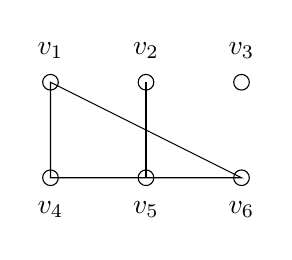
\begin{tikzpicture}[
            node distance=1cm,
            every node/.append style={circle,draw,inner sep=2pt}
        ]
            \node (A)            [label=above:$v_1$] {};
            \node (B) [right=of A,label=above:$v_2$] {};
            \node (C) [right=of B,label=above:$v_3$] {};
            \node (D) [below=of A,label=below:$v_4$] {};
            \node (E) [below=of B,label=below:$v_5$] {};
            \node (F) [below=of C,label=below:$v_6$] {};
            \draw (A.center) -- (F.center) -- (D.center) -- cycle;
            \draw (B.center) -- (E.center);
        \end{tikzpicture}
        \caption{The graph $\G$.}
        \label{fig:setgraph}
    \end{figure}
    \begin{itemize}
        \item Normally, a graph is represented by a picture as opposed to its formal set definition.
        \item For example, the graph $\G$ with vertex set $$\V=\left\{ v_1,v_2,v_3,v_4,v_5,v_6 \right\}$$ and edge set $$\E=\left\{ v_1v_4,v_1v_6,v_2v_5,v_4v_5,v_5v_6 \right\}$$ can be represented by Figure \ref{fig:setgraph}.
    \end{itemize}
    \item The above definition of a graph does not allow for \textbf{multiple edges} or \textbf{loops}, such as those in Figure \ref{fig:cubesgraph}.
    \begin{itemize}
        \item This is because most graphs of interest do not have these features.
    \end{itemize}
    \item \textbf{Multiple edges}: \dq{Several edges incident with the same two vertices}{bib:graph}{286}
    \item \textbf{Loop}: \dq{An edge which is incident with only one vertex}{bib:graph}{286}
    \item \textbf{Pseudograph}: A graph that may contain loops and/or multiple edges.
    \item Note that loops are counted twice when calculating degree --- for instance, vertex \Gre\ in Figure \ref{fig:cubesgraph} has $\deg {\color{green!30}G}=6$.
    \item There is no standard set of definitions of terms and symbols in graph theory, so make sure to check the glossary from book to book.
    \item \textbf{Subgraph} (of $\G$): A graph $\G_1$ such that its vertex and edge sets are, respectively, subsets of the vertex and edge sets of $\G$.
    \begin{itemize}
        \item Subgraphs do not have to be drawn in the same manner as the original graph.
    \end{itemize}
    \item Denoting deletions:
    \begin{itemize}
        \item For the graph $\G$ containing edge $e$, the subgraph $\G_1$ without $e$ will be denoted $\G\ \backslash\ \{e\}$ herein.
        \item For the graph $\G$ containing vertex $v$, the subgraph $\G_1$ without $v$ will be denoted $\G\ \backslash\ \{v\}$ herein.
        \item Note that if the vertex $v$ is deleted, all edges incident with $v$ must also be deleted.
    \end{itemize}
    \begin{figure}[h!]
        \centering
        \begin{subfigure}[b]{0.1\linewidth}
            \centering
            
\begin{tikzpicture}
                \node [circle,draw,inner sep=2pt] {};
            \end{tikzpicture}
            \caption{$\K_1$}
            \label{fig:5completesa}
        \end{subfigure}
        \begin{subfigure}[b]{0.1\linewidth}
            \centering
            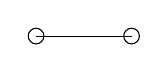
\begin{tikzpicture}[
                node distance=1cm,
                every node/.append style={circle,draw,inner sep=2pt}
            ]
                \node (A)              {};
                \node (B) [right=of A] {};
                \draw (A.center) -- (B.center);
            \end{tikzpicture}
            \caption{$\K_2$}
            \label{fig:5completesb}
        \end{subfigure}
        \begin{subfigure}[b]{0.1\linewidth}
            \centering
            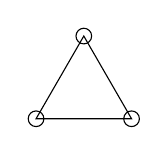
\begin{tikzpicture}[
                node distance=1cm,
                every node/.append style={circle,draw,inner sep=2pt}
            ]
                \node (A)                                   {};
                \node (B) [right=of A]                      {};
                \node (C) at ($(A.center)!1!60:(B.center)$) {};
                \draw (A.center) -- (B.center) -- (C.center) -- cycle;
            \end{tikzpicture}
            \caption{$\K_3$}
            \label{fig:5completesc}
        \end{subfigure}
        \begin{subfigure}[b]{0.1\linewidth}
            \centering
            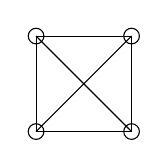
\begin{tikzpicture}[
                node distance=1cm,
                every node/.append style={circle,draw,inner sep=2pt}
            ]
                \node (A)              {};
                \node (B) [right=of A] {};
                \node (C) [above=of B] {};
                \node (D) [above=of A] {};
                \draw (A.center) -- (B.center) -- (C.center) -- (D.center) -- cycle;
                \draw (A.center) -- (C.center);
                \draw (B.center) -- (D.center);
            \end{tikzpicture}
            \caption{$\K_4$}
            \label{fig:5completesd}
        \end{subfigure}
        \begin{subfigure}[b]{0.15\linewidth}
            \centering
            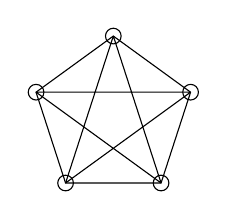
\begin{tikzpicture}[
                node distance=1cm,
                every node/.append style={circle,draw,inner sep=2pt},
                miter limit=3
            ]
                \node (A)                                     {};
                \node (B) [right=of A]                        {};
                \node (C) at ($(B.center)!1!-108:(A.center)$) {};
                \node (D) at ($(C.center)!1!-108:(B.center)$) {};
                \node (E) at ($(A.center)!1!108:(B.center)$)  {};
                \draw (A.center) -- (B.center) -- (C.center) -- (D.center) -- (E.center) -- cycle;
                \draw (B.center) -- (D.center) -- (A.center) -- (C.center) -- (E.center) -- cycle;
            \end{tikzpicture}
            \caption{$\K_5$}
            \label{fig:5completese}
        \end{subfigure}
        \caption{The first five complete graphs.}
        \label{fig:5completes}
    \end{figure}
    \item \textbf{Complete} (graph of $n$ vertices): The graph with $n$ vertices where any two vertices are adjacent. \emph{Also known as} $\K_n$.
    \begin{figure}[h!]
        \centering
        \begin{subfigure}[b]{0.2\linewidth}
            \centering
            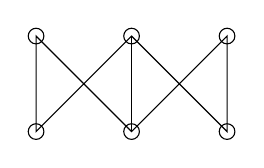
\begin{tikzpicture}[
                node distance=1cm,
                every node/.append style={circle,draw,inner sep=2pt}
            ]
                \node (A)              {};
                \node (B) [right=of A] {};
                \node (C) [right=of B] {};
                \node (D) [above=of C] {};
                \node (E) [above=of B] {};
                \node (F) [above=of A] {};
                \draw (A.center) -- (E.center) -- (C.center) -- (D.center) -- (B.center) -- (F.center) -- cycle;
                \draw (B.center) -- (E.center);
            \end{tikzpicture}
            \caption{A bipartite graph.}
            \label{fig:3bipartitesa}
        \end{subfigure}
        \begin{subfigure}[b]{0.2\linewidth}
            \centering
            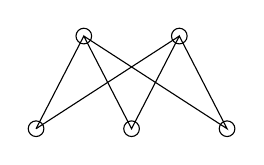
\begin{tikzpicture}[
                node distance=1cm,
                every node/.append style={circle,draw,inner sep=2pt}
            ]
                \node (A)                                     {};
                \node (B) [right=of A]                        {};
                \node (C) [right=of B]                        {};
                \node (D) [above=of $(B)!0.5!(C)$,yshift=2pt] {};
                \node (E) [above=of $(A)!0.5!(B)$,yshift=2pt] {};
                \draw (A.center) -- (E.center) -- (B.center) -- (D.center) -- (C.center) -- (E.center);
                \draw (A.center) -- (D.center);
            \end{tikzpicture}
            \caption{$\K_{2,3}$.}
            \label{fig:3bipartitesb}
        \end{subfigure}
        \begin{subfigure}[b]{0.2\linewidth}
            \centering
            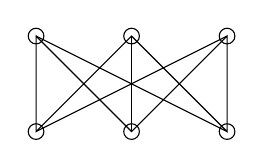
\begin{tikzpicture}[
                node distance=1cm,
                every node/.append style={circle,draw,inner sep=2pt}
            ]
                \node (A)              {};
                \node (B) [right=of A] {};
                \node (C) [right=of B] {};
                \node (D) [above=of C] {};
                \node (E) [above=of B] {};
                \node (F) [above=of A] {};
                \draw (A.center) -- (E.center) -- (C.center) -- (D.center) -- (B.center) -- (F.center) -- cycle;
                \draw (B.center) -- (E.center);
                \draw (A.center) -- (D.center);
                \draw (C.center) -- (F.center);
            \end{tikzpicture}
            \caption{$\K_{3,3}$.}
            \label{fig:3bipartitesc}
        \end{subfigure}
        \caption{Three bipartite graphs, two of which are complete bipartite.}
        \label{fig:3bipartites}
    \end{figure}
    \item \textbf{Bipartite} (graph): A graph whose vertices can be partitioned into two (disjoint) sets $\V_1$ and $\V_2$ such that every edge joins a vertex in $\V_1$ with a vertex in $\V_2$.
    \begin{itemize}
        \item These sets are called \textbf{bipartition sets}.
        \item A graph that can be drawn such that no two top vertices are adjacent and no two bottom vertices are adjacent.
    \end{itemize}
    \item \textbf{Complete bipartite} (graph): A bipartite graph in which every vertex $v\in\V_1$ is incident with every vertex $w\in\V_2$.
    \begin{itemize}
        \item The complete bipartite graph with $m$ and $n$ vertices in each respective bipartition set $\V_1$ and $\V_2$ is denoted $\K_{m,n}$.
        \item A bipartite graph that can be drawn such that every top vertex is adjacent to every bottom vertex.
    \end{itemize}
    \item Note that $\K_1$ is technically bipartite since bipartition sets are not required to be nonempty.
    \item Note that a graph is bipartite \dq{if and only if its vertices can be colored with two colors such that every edge has ends of different colors}{bib:graph}{289}
    \item A bipartite graph can contain no \textbf{triangles}.
    \item \textbf{Triangle} (in a graph): A set of three vertices with an edge joining each pair.
    \item \dq{The sum of the degrees of the vertices of a pseudograph is an even number equal to twice the number of edges}{bib:graph}{290} Symbolically, if $\G(\V,\E)$ is a pseudograph, then the following holds.
    \begin{equation*}
        \sum_{v\in\V}\deg v=2|\E|
    \end{equation*}
    \begin{itemize}
        \item Because each edge gets counted twice --- once at each vertex it touches. A loop gets counted twice for the same vertex.
        \item Example: How many edges does $\K_{m,n}$ have?
        \begin{itemize}
            \item $\K_{m,n}$ has $m$ vertices of degree $n$ and $n$ vertices of degree $m$. Therefore,
            \begin{equation*}
                \sum_{v\in\V}\deg v=mn+nm=2mn=2|\E|
            \end{equation*}
            so the number of edges is equal to $m\times n$.
        \end{itemize}
    \end{itemize}
    \item \textbf{Degree sequence} (of $\G$): The degrees $d_1,\dots,d_n$ of the vertices $v_1,\dots,v_n$ of a graph (or pseudograph) $\G$ ordered such that $d_1\geq\dots\geq d_n$.
    \item \dq{The number of odd vertices in a pseudograph is even}{bib:graph}{290}
    \begin{itemize}
        \item The sum of the degrees of the vertices of a pseudograph is an even number, and the sum of the degrees of the even vertices is an even number. Thus, the sum of the degrees of the odd vertices must be even. Since only the sum of an even number of odd numbers is even, there must be an even number of odd vertices.
    \end{itemize}
\end{itemize}


\subsection{Isomorphism}
\begin{itemize}
    \item There is a distinction between a graph and its picture because a graph is pair of sets whereas its picture can be drawn many different ways.
    \begin{figure}[h!]
        \centering
        \footnotesize
        \begin{subfigure}[b]{0.15\linewidth}
            \centering
            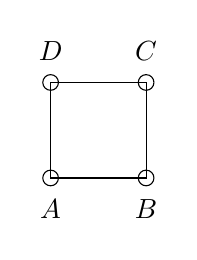
\begin{tikzpicture}[
                node distance=1cm,
                every node/.append style={circle,draw,inner sep=2pt}
            ]
                \node (A)            [label=below:$A$] {};
                \node (B) [right=of A,label=below:$B$] {};
                \node (C) [above=of B,label=above:$C$] {};
                \node (D) [above=of A,label=above:$D$] {};
                \draw (A.center) -- (B.center) -- (C.center) -- (D.center) -- cycle;
            \end{tikzpicture}
            \caption{$\G_1$.}
            \label{fig:isomorphica}
        \end{subfigure}
        \begin{subfigure}[b]{0.15\linewidth}
            \centering
            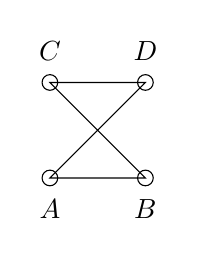
\begin{tikzpicture}[
                node distance=1cm,
                every node/.append style={circle,draw,inner sep=2pt}
            ]
                \node (A)            [label=below:$A$] {};
                \node (B) [right=of A,label=below:$B$] {};
                \node (C) [above=of A,label=above:$C$] {};
                \node (D) [above=of B,label=above:$D$] {};
                \draw (A.center) -- (B.center) -- (C.center) -- (D.center) -- cycle;
            \end{tikzpicture}
            \caption{$\G_2$.}
            \label{fig:isomorphicb}
        \end{subfigure}
        \begin{subfigure}[b]{0.15\linewidth}
            \centering
            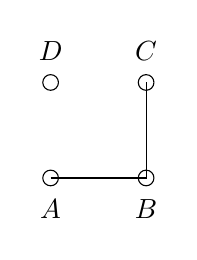
\begin{tikzpicture}[
                node distance=1cm,
                every node/.append style={circle,draw,inner sep=2pt}
            ]
                \node (A)            [label=below:$A$] {};
                \node (B) [right=of A,label=below:$B$] {};
                \node (C) [above=of B,label=above:$C$] {};
                \node (D) [above=of A,label=above:$D$] {};
                \draw (A.center) -- (B.center) -- (C.center);
            \end{tikzpicture}
            \caption{$\G_3$.}
            \label{fig:isomorphicc}
        \end{subfigure}
        \caption{$\G_1$ and $\G_2$ are isomorphic, but neither is isomorphic to $\G_3$.}
        \label{fig:isomorphic}
    \end{figure}
    \item \textbf{Isomorphic} (graphs): Two graphs $\G_1=\G_1(\V_1,\E_1)$ and $\G_2=\G_2(\V_2,\E_2)$ such that there exists a one-to-one function $\varphi$ from $\V_1$ onto $\V_2$ such that\dots
    \begin{itemize}
        \item if $vw$ is an edge in $\E_1$, then $\varphi(v)\varphi(w)$ is an edge in $\E_2$, and
        \item every edge in $\E_2$ has the form $\varphi(v)\varphi(w)$ for some edge $vw\in\E_1$.
    \end{itemize}
    \item \textbf{Isomorphism}: A one-to-one function $\varphi$ from $\G_1$ to $\G_2$.
    \item Two isomorphic graphs $\G_1$ and $\G_2$ are denoted $\G_1\cong\G_2$.
    \item An isomorphism from $\G_1$ to $\G_2$ is denoted (herein) $\varphi:\G_1\rightarrow\G_2$.
    \item The definition of isomorphism is naturally symmetric --- $\G_1\cong\G_2\Rightarrow\G_2\cong\G_1$.
    \item Likewise, $\varphi:\G_1\rightarrow\G_2\Rightarrow\varphi^{-1}:\G_2\rightarrow\G_1$.
    \item To avoid ambiguity, say that two graphs "are isomorphic."
    \item Isomorphisms relabel vertices without changing any incidence relations, i.e., two graphs are isomorphic if and only if there exists a \textbf{bijection} between their sets that "preserves incidence relations."
    \item Isomorphisms can be written down explicitly.
    \begin{figure}[h!]
        \centering
        \begin{subfigure}[b]{0.15\linewidth}
            \centering
            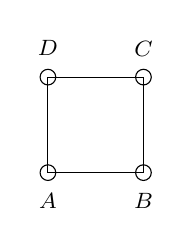
\begin{tikzpicture}[
                node distance=1cm,
                every node/.append style={circle,draw,inner sep=2pt}
            ]
                \footnotesize
                \node (A)            [label=below:$A$] {};
                \node (B) [right=of A,label=below:$B$] {};
                \node (C) [above=of B,label=above:$C$] {};
                \node (D) [above=of A,label=above:$D$] {};
                \draw (A.center) -- (B.center) -- (C.center) -- (D.center) -- cycle;
            \end{tikzpicture}
            \caption{$\G_1$.}
            \label{fig:isomorphisma}
        \end{subfigure}
        \begin{subfigure}[b]{0.15\linewidth}
            \centering
            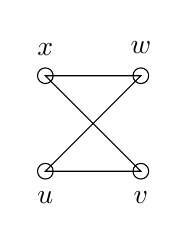
\begin{tikzpicture}[
                node distance=1cm,
                every node/.append style={circle,draw,inner sep=2pt}
            ]
                \node (A)            [label=below:$u$] {};
                \node (B) [right=of A,label=below:$v$] {};
                \node (C) [above=of A,label=above:$x$] {};
                \node (D) [above=of B,label=above:$w$] {};
                \draw (A.center) -- (B.center) -- (C.center) -- (D.center) -- cycle;
            \end{tikzpicture}
            \caption{$\G_2$.}
            \label{fig:isomorphismb}
        \end{subfigure}
        \caption{Isomorphisms as explicit functions.}
        \label{fig:isomorphism}
    \end{figure}
    \begin{itemize}
        \item The isomorphism between the vertices in Figures \ref{fig:isomorphisma} and \ref{fig:isomorphismb} (recall Figures \ref{fig:isomorphica} and \ref{fig:isomorphicb}) can be denoted as follows.
        \begin{equation*}
            \varphi(u)=A,\ \varphi(v)=B,\ \varphi(w)=D,\ \varphi(x)=C
        \end{equation*}
    \end{itemize}
    \item Isomorphisms are very important in mathematics.
    \begin{itemize}
        \item Although the term "isomorphism" may be new, the concept is not --- $0.5$ and $\frac{2}{4}$ are isomorphic objects.
        \item They are \textbf{symmetric}, as previously mentioned.
        \item They are also \textbf{reflexive}: $\G\cong\G$ for any graph $\G$.
        \begin{itemize}
            \item Because the map $\G\rightarrow\G$ (an identity) is an isomorphism.
        \end{itemize}
        \item They are also \textbf{transitive}: $\G_1\cong\G_2\textsc{ and }\G_2\cong\G_3\Rightarrow\G_1\cong\G_3$.
        \begin{itemize}
            \item Because if $\varphi_1:\G_1\rightarrow\G_2$ and $\varphi_2:\G_2\rightarrow\G_3$ are isomorphisms, then so is the composition $\varphi_1\circ\varphi_2:\G_1\rightarrow\G_3$.
        \end{itemize}
    \end{itemize}
    \item The set of all graphs is partitioned into disjoint equivalence classes known as \textbf{isomorphism classes}.
    \item \textbf{Isomorphism class}: The set of all graphs $\G$ that are isomorphic to one another.
    \begin{itemize}
        \item In Figure \ref{fig:isomorphic}, $\G_1$ and $\G_2$ are in the same isomorphism class while $\G_1$ and $\G_3$, and $\G_2$ and $\G_3$ are not.
    \end{itemize}
    \item It is often difficult to prove that graphs are isomorphic, but easy to prove that they are not.
    \item \dq{If $\G_1$ and $\G_2$ are isomorphic graphs, then $\G_1$ and $\G_2$ have the
    \begin{itemize}
        \item same number of vertices,
        \item same number of edges, and
        \item same degree sequences}{bib:graph}{297}
    \end{itemize}
    \item Note that the converses of the above qualities are not necessarily true --- two graphs with the same number of vertices are not necessarily isomorphic.
\end{itemize}
\newpage



\section{Applications}
\subsection{Graphs and Networks}
From \cite{bib:Strang}.
\begin{itemize}
    \item Goal is to show how graphs illuminate the Fundamental Theorem of Linear Algebra.
    \item \textbf{Incidence matrix} (of a graph): A matrix describing how $n$ nodes (of a graph) are connected by $m$ edges.
    \begin{itemize}
        \item \dq{Every entry of an incidence matrix is a $0$ or $1$ or $-1$}{bib:Strang}{420}
        \item Because of this, all four subspaces and reduced versions also have only these three entries.
    \end{itemize}
    \begin{align*}
        A &=
        \begin{bmatrix}
            -1 & 1  & 0  & 0\\
            -1 & 0  & 1  & 0\\
            0  & -1 & 1  & 0\\
            -1 & 0  & 0  & 1\\
            0  & -1 & 0  & 1\\
            0  & 0  & -1 & 1
        \end{bmatrix}
        &
        U &=
        \begin{bmatrix}
            -1 & 1  & 0  & 0\\
            0  & -1 & 1  & 0\\
            0  & 0  & -1 & 1\\
            0  & 0  & 0  & 0\\
            0  & 0  & 0  & 0\\
            0  & 0  & 0  & 0
        \end{bmatrix}
    \end{align*}
    \item Consider the example incidence matrix above and its upper-triangular equivalent.
    \begin{itemize}
        \item $C(A)=\left\{
        \begin{bmatrix}
            -1\\
            -1\\
            0\\
            -1\\
            0\\
            0
        \end{bmatrix},
        \begin{bmatrix}
            1\\
            0\\
            -1\\
            0\\
            -1\\
            0
        \end{bmatrix},
        \begin{bmatrix}
            0\\
            1\\
            1\\
            0\\
            0\\
            -1
        \end{bmatrix}
        \right\}$
        \item $C(A^\T)=\left\{
        \begin{bmatrix}
            -1\\
            1\\
            0\\
            0
        \end{bmatrix},
        \begin{bmatrix}
            0\\
            -1\\
            1\\
            0
        \end{bmatrix},
        \begin{bmatrix}
            0\\
            0\\
            -1\\
            1
        \end{bmatrix}
        \right\}$
        \item $N(A)=\left\{
        \begin{bmatrix}
            1\\
            1\\
            1\\
            1
        \end{bmatrix}
        \right\}$
        \item Every vector in $N(A)$ is perpendicular to every vector in $C(A^\T)$, i.e., the subspaces are orthogonal (see Figure \ref{fig:4spaces}).
        \begin{figure}[h!]
            \centering
            \begin{tikzpicture}[
                node distance=0pt,
                recta/.style n args={4}{draw,shape=trapezium,trapezium left angle=90,shape border uses incircle,trapezium right angle=90,shape border rotate=#1,trapezium stretches=true,minimum width=#2,minimum height=#3,align=center,text width=#4}
            ]
                \begin{scope}
                    \node (a) [recta={45}{4cm}{3cm}{1cm},label=120:$\dim r$] {row space of $A$};
                    \node (b) [recta={-45}{3cm}{0cm}{1.5cm},label=-120:$\dim n-r$,label=104:$\R^n$,below=3.65mm of a.-94] {nullspace of $A$};
                    \clip (a.-80) -- (a.-98) -- (b.80);
                    \node [recta={45}{6mm}{6mm}{0cm}] at (a.-98) {};
                \end{scope}
                \begin{scope}[xshift=10cm]
                    \node (c) [recta={120}{4cm}{3cm}{1.5cm},label=60:$\dim r$] {column space of $A$};
                    \node (d) [recta={30}{3cm}{0cm}{1.5cm},label=-60:$\dim m-r$,label=58:$\R^m$,below=15.5mm of c.-127,xshift=-0.1pt] {nullspace of $A^\T$};
                    \clip (c.-105) -- (c.-97) -- (d.90);
                    \node [recta={30}{6mm}{6mm}{0cm}] at (c.-97) {};
                \end{scope}
            \end{tikzpicture}
            \caption{The four subspaces with their dimensions and orthogonality.}
            \label{fig:4spaces}
        \end{figure}
        \begin{itemize}
            \item This is demonstrated by the fact that the dot product of every basis vector with every other basis vector between subspaces is 0.
        \end{itemize}
        \item The implication of this is that \dq{equal voltages produce no current}{bib:Strang}{420}
    \end{itemize}
    \item \textbf{Column space} (of an $m$ by $n$ matrix $A$): The linear combinations of the column vectors of $A$. A subspace of $\R^m$. Exactly all possible matrix-vector products $Ax$. \emph{Also known as} $C(A)$.
    \item \textbf{Row space} (of an $m$ by $n$ matrix $A$): The linear combinations of the row vectors (the column vectors of $A^\T$). A subspace of $\R^n$. Exactly all possible matrix-vector products $A^\T x$. \emph{Also known as} $C(A^\text{T})$.
    \item \textbf{Nullspace} (of an $m$ by $n$ matrix $A$): A subspace of $\R^n$ containing every $x$ that satisfies $Ax=0$. \emph{Also known as} $N(A)$.
    \item \textbf{Left nullspace} (of an $m$ by $n$ matrix $A$): A subspace of $\R^m$ containing every $y$ that satisfies $A^\T y-0$. So named because, when written $y^\T A=0^T$ (with $y^\T$ to the left of $A$), $y$ combines the rows of $A$. \emph{Also known as} $N(A^\T)$.
    \item \textbf{Dimension} (of a vector space $V$): A function that gives the number of basis vectors of $V$. \emph{Also known as} $\dim V$.
    \item Two central laws of linear algebra:
    \begin{itemize}
        \item $\dim C(A)=\dim C(A^\T)$
        \item $\dim C(A)+\dim N(A)=n$
    \end{itemize}
    \begin{figure}[h!]
        \centering
        \begin{subfigure}[b]{0.4\linewidth}
            \centering
            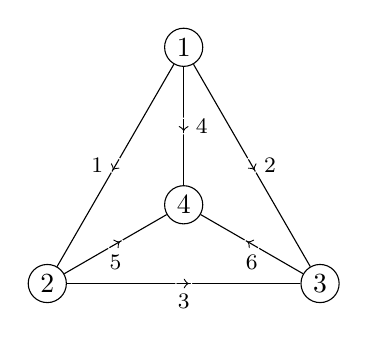
\begin{tikzpicture}[
                every node/.style={circle,draw,inner sep=2pt},
                every edge/.append style={decoration={markings,
                    mark=at position 0.5 with \arrow{<}
                },postaction={decorate}},
                label distance=-1mm
            ]
                \node (1) at (90:2)   {1};
                \node (2) at (-150:2) {2}
                    edge node[draw=white,label=left:{\footnotesize1}] {} (1)
                ;
                \node (3) at (-30:2)  {3}
                    edge node[draw=white,label=right:{\footnotesize2}]{} (1)
                    edge node[draw=white,label=below:{\footnotesize3}]{} (2)
                ;
                \node (4)             {4}
                    edge node[draw=white,label=right:{\footnotesize4}]{} (1)
                    edge node[draw=white,label=below:{\footnotesize5}]{} (2)
                    edge node[draw=white,label=below:{\footnotesize6}]{} (3)
                ;
            \end{tikzpicture}
            \caption{A directed graph.}
            \label{fig:compgraphincia}
        \end{subfigure}
        \begin{subfigure}[b]{0.4\linewidth}
            \centering
            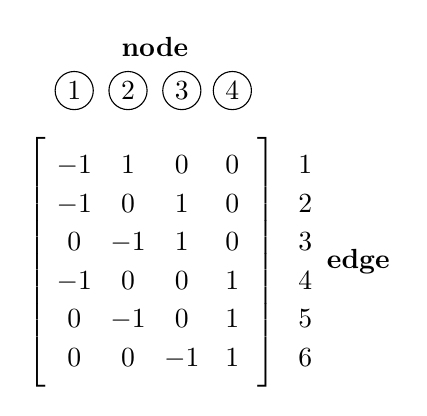
\begin{tikzpicture}[
                every left delimiter/.style={xshift=1ex},
                every right delimiter/.style={xshift=-1ex}
            ]
                \matrix (m) [nodes={minimum width=6mm},matrix of math nodes,left delimiter={[},right delimiter={]}] {
                    -1 & 1  & 0  & 0\\
                    -1 & 0  & 1  & 0\\
                    0  & -1 & 1  & 0\\
                    -1 & 0  & 0  & 1\\
                    0  & -1 & 0  & 1\\
                    0  & 0  & -1 & 1\\
                };
                \foreach \x in {1,2,3,4} {
                    \node [circle,draw,node distance=3ex,inner sep=2pt,above=of m-1-\x] {\x};
                }
                \node at ([yshift=15mm]$(m-1-2)!0.5!(m-1-3)$) {\textbf{node}};
                \foreach \y in {1,...,6} {
                    \node [node distance=3ex,inner sep=2pt,right=of m-\y-4] {\y};
                }
                \node at ([xshift=16mm]$(m-3-4)!0.5!(m-4-4)$) {\textbf{edge}};
            \end{tikzpicture}
            \caption{An incidence matrix.}
            \label{fig:compgraphincib}
        \end{subfigure}
        \caption{A complete graph ($\K_4$) and its incidence matrix.}
        \label{fig:compgraphinci}
    \end{figure}
    \item Because the graph in Figure \ref{fig:compgraphincia} has 4 nodes and 6 edges, the incidence matrix in Figure \ref{fig:compgraphincib} has $m=6$ and $n=4$.
    \item The values in row 1 mean that edge 1 flows out of node 1 and into node 2.
    \item \textbf{Directed graph}: A graph where all edges have an associated direction.
    \begin{figure}[h!]
        \centering
        \begin{subfigure}[b]{0.4\linewidth}
            \centering
            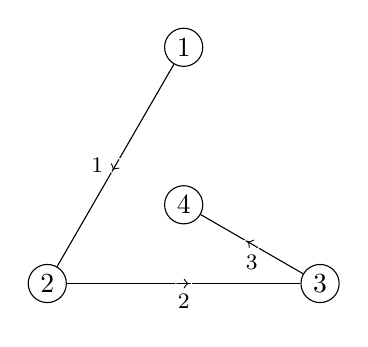
\begin{tikzpicture}[
                every node/.style={circle,draw,inner sep=2pt},
                every edge/.append style={decoration={markings,
                    mark=at position 0.5 with \arrow{<}
                },postaction={decorate}},
                label distance=-1mm
            ]
                \node (1) at (90:2)   {1};
                \node (2) at (-150:2) {2}
                    edge node[draw=white,label=left:{\footnotesize1}] {} (1)
                ;
                \node (3) at (-30:2)  {3}
                    edge node[draw=white,label=below:{\footnotesize2}]{} (2)
                ;
                \node (4)             {4}
                    edge node[draw=white,label=below:{\footnotesize3}]{} (3)
                ;
            \end{tikzpicture}
            \caption{A tree with no loops.}
            \label{fig:compgraphrefa}
        \end{subfigure}
        \begin{subfigure}[b]{0.4\linewidth}
            \centering
            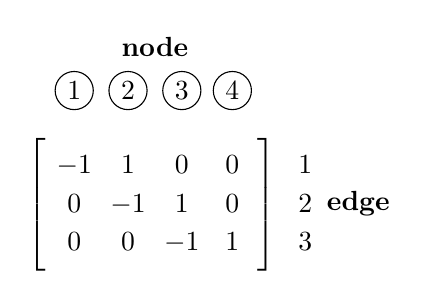
\begin{tikzpicture}[
                every left delimiter/.style={xshift=1ex},
                every right delimiter/.style={xshift=-1ex}
            ]
                \matrix (m) [nodes={minimum width=6mm},matrix of math nodes,left delimiter={[},right delimiter={]}] {
                    -1 & 1  & 0  & 0\\
                    0  & -1 & 1  & 0\\
                    0  & 0  & -1 & 1\\
                };
                \foreach \x in {1,2,3,4} {
                    \node [circle,draw,node distance=3ex,inner sep=2pt,above=of m-1-\x] {\x};
                }
                \node at ([yshift=15mm]$(m-1-2)!0.5!(m-1-3)$) {\textbf{node}};
                \foreach \y in {1,...,3} {
                    \node [node distance=3ex,inner sep=2pt,right=of m-\y-4] {\y};
                }
                \node at ([xshift=16mm]m-2-4) {\textbf{edge}};
            \end{tikzpicture}
            \caption{$\text{ref}(A)$.}
            \label{fig:compgraphrefb}
        \end{subfigure}
        \caption{The tree corresponding to the row eschelon form of the previous incidence matrix.}
        \label{fig:compgraphref}
    \end{figure}
    \item \textbf{Tree}: A graph with no closed loops.
    \item The setups in Figure \ref{fig:compgraphinci} and \ref{fig:compgraphref} are opposites --- the former has the maximum number of edges ($\frac{1}{2}n(n-2)$) while the latter has the minimum ($m=n-1$).
    \item \dq{Elimination reduces every graph to a tree}{bib:Strang}{423}
    \item Row space:
    \begin{itemize}
        \item When edges form a loop, some rows must be dependent.
        \item Independent rows come from trees.
        \item Flow along the arrow counts as positive while flow against the arrow counts as negative.
    \end{itemize}
    \item Column space:
    \begin{equation*}
        Ax=
        \begin{bmatrix}
            -1 & 1  & 0  & 0\\
            -1 & 0  & 1  & 0\\
            0  & -1 & 1  & 0\\
            -1 & 0  & 0  & 1\\
            0  & -1 & 0  & 1\\
            0  & 0  & -1 & 1
        \end{bmatrix}
        \begin{bmatrix}
            x_1\\
            x_2\\
            x_3\\
            x_4
        \end{bmatrix}
        =
        \begin{bmatrix}
            x_2-x_1\\
            x_3-x_1\\
            x_3-x_2\\
            x_4-x_1\\
            x_4-x_2\\
            x_4-x_3
        \end{bmatrix}
    \end{equation*}
    \begin{itemize}
        \item The unknowns in the $x$ vector represent voltages or potentials.
        \item The unknowns in the $Ax$ vector represent voltage differences or potential difference across the edges.
        \item These differences cause flows.
        \item \textbf{Kirchoff's voltage law}: \dq{The components of $Ax$ add to zero around every loop}{bib:Strang}{426}
    \end{itemize}
    \item Meaning of the nullspace:
    \begin{itemize}
        \item When all four potentials are equal, there is no current.
        \item The potentials can be raised and lowered by $\begin{bmatrix}c\\c\\c\\c\end{bmatrix}$ without changing the differences.
        \begin{itemize}
            \item Similar to how $f(x)$ can be raised and lowered by $C$ without changing its derivative.
        \end{itemize}
        \item Linear algebra adds $x_n$ to a particular solution.
        \begin{itemize}
            \item Calculus adds $C$ to a particular solution of an integral.
        \end{itemize}
        \item The nullspace disappears when any value of $x$ is set to a constant.
        \begin{itemize}
            \item $C$ disappears during a definite integral.
        \end{itemize}
    \end{itemize}
    \item \textbf{Grounding} (a node): Removing a node.
    \item Meaning of the row space:
    \begin{itemize}
        \item $v$ is in the row space if and only if it is perpendicular to $\begin{bmatrix}1\\1\\1\\1\end{bmatrix}$ in the nullspace.
        \item The values of any vector in the row space sum to zero.
    \end{itemize}
    \item Meaning of the column space:
    \begin{itemize}
        \item \dq{The components of $Ax$ add to zero around every loop}{bib:Strang}{424}
        \item When $b$ is in the column space of $A$, it must obey Kirchoff's Law, which follows.
        \begin{equation*}
            b_1+b_3-b_2=0
        \end{equation*}
    \end{itemize}
    \item Meaning of the left nullspace:
    \begin{equation*}
        A^\T y=
        \begin{bmatrix}
            -1 & -1 & 0  & -1 & 0  & 0 \\
            1  & 0  & -1 & 0  & -1 & 0 \\
            0  & 1  & 1  & 0  & 0  & -1\\
            0  & 0  & 0  & 1  & 1  & 1
        \end{bmatrix}
        \begin{bmatrix}
            y_1\\
            y_2\\
            y_3\\
            y_4\\
            y_5\\
            y_6
        \end{bmatrix}
        =
        \begin{bmatrix}
            0\\
            0\\
            0\\
            0
        \end{bmatrix}
    \end{equation*}
    \begin{itemize}
        \item Components of $y$ ($y_n$) are currents.
        \item \dq{When currents or forces are in equilibrium, the equation to solve is $A^\T y=0$}{bib:Strang}{425}
        \item The first row in $A^\T$ gives all edges (currents) that interact with node 1, namely, edges 1, 2, and 4 flowing out.
        \item That these edges times a vector in the left null space equals zero means that the net flow into node 1 is zero.
        \begin{itemize}
            \item The same holds true for all other nodes (as shown by the other rows in $A^\T$).
            \item This gives \textbf{Kirchoff's Current Law}.
        \end{itemize}
        \item \textbf{Kirchoff's Current Law}: \dq{Flow in equals flow out at each node}{bib:Strang}{425}
        \item Let's interpret this: a loop current is a loop of edges, such as edges 1, 2, and 3 in Figure \ref{fig:compgraphincia}.
        \begin{itemize}
            \item To get around this loop, flow forward on edge 1 (from node 1 to 2), forward on edge 2 (from node 2 to 3), and backward on edge 3 (from node 3 to 1).
            \item This progression can be expressed by the vector, $\begin{bmatrix}1\\-1\\1\\0\\0\\0\end{bmatrix}$.
            \item Indeed, this vector is a viable $y$ vector.
            \item In fact, \dq{every loop current is a solution to the current law}{bib:Strang}{425}
        \end{itemize}
        \item Since $\dim m-r=6-3=3$, we expect 3 independent left null space vectors.
        \begin{itemize}
            \item These can be found via tracing independent loops in Figure \ref{fig:compgraphincia}.
            \item To ensure independence of loops, choose any three values $y_n$ and have each loop include only one of these edges.
            \item For instance, choose edges $y_1$, $y_2$, and $y_3$, or edges 1, 2, and 3.
            \item The first loop will therefore include edge 1 and some set of edges 4, 5, and 6. For simplicity's sake, choose edges 4 and 5.
            \item Do something similar to find the other two loops to include edges 2, 4, and 6, and edges 3, 5, and 6.
            \item Tracing the flow along these edges gives the following basis.
            \item $N(A^\T)=\left\{
            \begin{bmatrix}
                1\\
                0\\
                0\\
                -1\\
                1\\
                0
            \end{bmatrix},
            \begin{bmatrix}
                0\\
                0\\
                1\\
                0\\
                -1\\
                1
            \end{bmatrix},
            \begin{bmatrix}
                0\\
                -1\\
                0\\
                1\\
                0\\
                -1
            \end{bmatrix}
            \right\}$
            \item Note that the sum of these vectors gives the one for the big loop listed previously.
        \end{itemize}
    \end{itemize}
    \item Given an $m\times n$ incidence matrix, $r=n-1$, using edges from any tree.
    \item There are $m-r=m-n+1$ independent loops in a graph.
    \item Every graph testifies to \textbf{Euler's formula}$^[$\footnote{The same idea as the Euler characteristic from Section 4.1 in \cite{bib:knotnotes}.}$^]$.
    \item \textbf{Euler's formula}: $(\text{number of nodes})-(\text{number of edges})+(\text{number of small loops})=1$
    \begin{itemize}
        \item Simply proven: $n-m+(m-n+1)=1$.
    \end{itemize}
    \item In real life, the current $y$ is the product of the difference in potentials $Ax$ and the \textbf{conductance} $c$.
    \item \textbf{Conductance}: A measure of how easily flow passes through an edges.
    \item A "connectivity matrix" $A$ (an incidence matrix) describes the connections in a graph.
    \item A \textbf{network} assigns a conductance to each edge. These numbers ($c_1,\dots,c_m$) go into the "conductance matrix" $C$.
    \item $\text{conductance}=\frac{1}{\text{resistance}}$.
    \item \textbf{Ohm's Law}: $\text{Current along edge}=\text{conductance}\times\text{potential difference}$.
    \item Therefore, \dq{Ohm's Law for all $m$ currents is $y=-CAx$}{bib:Strang}{426}
    \item Combining Ohm's Law and Kirchoff's Current Law yields $A^\T CAx=0$$^[$\footnote{In circuit theory, we do change from $Ax$ to $-Ax$.}$^]$.
    \item When there is a current source, Kirchoff's Current Law changes from $A^\T y=0$ to $A^\T y=f$. Flow is still balanced, but it is shifted.
    \item \textbf{Graph Laplacian matrix}: The matrix $A^\T A$$^[$\footnote{There is an example with these concepts, but it is beyond me for the time being.}$^]$.
\end{itemize}
\newpage



\section{Fundamental Concepts}
\subsection{Rings and Fields}
From \cite{bib:determinants}.
\begin{itemize}
    \item \textbf{Ring}: A set $\mathfrak{R}$ of elements $a,b,c,\dots$ along with two rules of combination (addition and multiplication) such that if $a,b\in\mathfrak{R}$, then $a+b$ and $ab$ are uniquely defined elements of $\mathfrak{R}$.
    \begin{itemize}
        \item A ring is a generalization of a vector field.
        \item Rings are algebraic structures while vector fields are geometric structures.
        \item Rings are studied in abstract algebra.
    \end{itemize}
    \item Addition and multiplication obey the following five laws, which are very similar to those governing a vector field.
    \begin{description}
        \item[commutative law of addition] \hfill \\ $a+b=b+a$
        \item[associative law of addition] \hfill \\ $a+(b+c)=(a+b)+c$
        \item[subtraction] \hfill \\ The equation $a+x=b$ always has a solution in $\mathfrak{R}$.
        \item[associative law of multiplication] \hfill \\ $a(bc)=(ab)c$
        \item[distributive laws] \hfill \\ $a(b+c)=ab+ac$ \hfill \\ $(b+c)a=ba+bc$
    \end{description}
    \item The law of subtraction is not postulated, but can be proved from the others.
    \begin{itemize}
        \item The unique solution is $x=b-a$.
    \end{itemize}
    \item \textbf{Commutative} (ring): A ring where $ab=ba$ is satisfied for $a,b\in\mathfrak{R}$ in addition to the above conditions.
    \item \textbf{Zero element}: A unique element 0 of every ring $\mathfrak{R}$ that has the following properties for every element $a\in\mathfrak{R}$.
    \begin{align*}
        a+0 &= 0+a = a\\
        a\times 0 &= 0\times a = 0
    \end{align*}
    \item \textbf{Right unity} (element): An element $e$ such that $ae=a$ for every $a\in\mathfrak{R}$.
    \item \textbf{Left unity} (element): An element $f$ such that $fa=a$ for every $a\in\mathfrak{R}$.
    \item If a ring has both a right unity element $e$ and a left unity element $f$, then $e=f$.
    \begin{itemize}
        \item By the definition of the right unity element, $fe=f$.
        \item By the definition of the left unity element, $fe=e$.
        \item Thus, $e=fe=f$.
        \item Therefore, $e=f$.
    \end{itemize}
    \item Examples of rings: $\mathbb{Z}$; $2\mathbb{Z}$; $a+b\sqrt{2}:a,b\in\mathbb{Z}$; $\mathbb{Q}$; the set of all polynomials in a single variable with real coefficients.
    \item \textbf{Field}: A ring $\mathfrak{F}$ such that the equation $ax=b$ has a solution where $x\in\mathfrak{F}$ for all $a,b\in\mathfrak{F}$.
    \begin{itemize}
        \item In a field, division, except by 0, is always possible.
        \item A field always has a unique unity element denoted 1 such that $a\times 1=a$.
        \item \dq{In a field if $ab=0$ and $a\neq 0$, then $b=0$}{bib:determinants}{4}
    \end{itemize}
\end{itemize}


\subsection{The Matrix}
\begin{itemize}
    \item \textbf{Matrix} (over the ring $\mathfrak{R}$): The rectangular array of $m$ rows and $n$ columns containing the elements $a_{11},a_{12},\dots,a_{mn}$ of ring $\mathfrak{R}$.
    \begin{equation*}
        A=
        \begin{bmatrix}
            a_{11} & a_{12} & \cdots & a_{1n}\\
            a_{21} & a_{22} & \cdots & a_{2n}\\
            \vdots & \vdots & \ddots & \vdots\\
            a_{m1} & a_{m2} & \cdots & a_{mn}
        \end{bmatrix}
    \end{equation*}
    \begin{itemize}
        \item Denoted by uppercase Latin letters ($A,B,C,\dots$).
        \item Also denoted in these two ways (examples correspond to the matrix $A$): $(a_{ij})$, $||a_{ij}||$.
    \end{itemize}
    \item \textbf{Dimensions} (of $A$): The values $m$ and $n$ corresponding to the number of rows and columns, respectively.
    \item \textbf{Diagonal} (elements): The elements $a_{11},a_{22},\dots$. \emph{Also known as} \textbf{the elements in the principal diagonal}.
    \item \textbf{\emph{n}-square matrix}: A matrix with $n$ rows and $n$ columns. \emph{Also known as} \textbf{square matrix of order \emph{n}}.
\end{itemize}


\subsection{Certain Operations with Matrices}
\begin{itemize}
    \item \textbf{Equal} (matrices over $\mathfrak{R}$): Two matrices $A$ and $B$ with elements in a ring $\mathfrak{R}$ that
    \begin{enumerate}
        \item have the same dimensions and
        \item satisfy $a_{ij}=b_{ij}\ \forall\ i=1,\dots,m;j=1,\dots,n$.
    \end{enumerate}
    \item \textbf{Zero} (matrix): A matrix where each element of is zero.
    \begin{itemize}
        \item Denoted by $A=0$.
    \end{itemize}
    \item \textbf{Sum} (of two $m\times n$ matrices $A$ and $B$): The $m\times n$ matrix $C$, every element of which satisfies $c_{ij}=a_{ij}+b_{ij}$.
    \item \textbf{Difference} (of two $m\times n$ matrices $A$ and $B$): The $m\times n$ matrix $C$, every element of which satisfies $c_{ij}=a_{ij}-b_{ij}$.
    \item \textbf{Scalar}: A single element of a ring $\mathfrak{R}$.
    \begin{itemize}
        \item Denoted by lowercase Latin or Greek letters ($a,b,c,\dots$ or $\alpha,\beta,\gamma,\dots$).
    \end{itemize}
    \item Establishes matrix properties based on those governing a commutative ring.
\end{itemize}


\subsection{Multiplication of Matrices}
\begin{itemize}
    \item \textbf{Product} (of an $m\times n$ matrix $A$ and an $n\times q$ matrix $B$ over $\mathfrak{R}$): The $m\times q$ matrix $C=AB$, every element of which satisfies $c_{ij}=\sum_{t=1}^n a_{it}b_{tj}$.
    \begin{itemize}
        \item If $\mathfrak{R}$ is commutative, then $c_{ij}=\sum_{t=1}^n a_{it}b_{tj}=\sum_{t=1}^n b_{tj}a_{it}$.
        \item If $\mathfrak{R}$ is not commutative, then $c_{ij}$ equals only $\sum_{t=1}^n a_{it}b_{tj}$.
    \end{itemize}
    \item If $AB$ exists, then $A$ and $B$ \dq{must have their \textbf{contiguous} dimensions equal}{bib:determinants}{6}. Another way of saying this is that $A$ and $B$ must be \textbf{conformable} for multiplication.
    \item \textbf{Contiguous} (dimensions): For two matrices $A$ and $B$, the dimensions that must be the same when multiplied if $AB$ exists.
    \item \textbf{Conformable} (matrices): Two matrices $A$ and $B$ for which the product $AB$ exists.
    \item \dq{If $A$ is an $m\times n$ matrix, $B$ and $C$ $n\times q$ matrices, then $A(B+C)=AB+AC$}{bib:determinants}{7}
    \begin{itemize}
        \item Because $B$ and $C$ are both $n\times q$ matrices, $B+C$ is $n\times q$.
        \item Thus, the matrices $A(B+C)$ and $AB+AC$ are both $m\times q$.
        \item Because $a_{ij},b_{ij},c_{ij}\in\mathfrak{R}$ and because of the distributive laws governing rings, $\sum_{t=1}^n a_{it}(b_{tj}+c_{tj}) = \sum_{t=1}^na_{it}b_{tj}+\sum_{t=1}^na_{it}c_{tj}$.
        \item Therefore, because the dimensions and elements of $A(B+C)$ and $AB+AC$ are equal, $A(B+C)=AB+AC$.
    \end{itemize}
    \item \dq{If $A$, $B$, and $C$ are three matrices of dimensions $m\times n$, $n\times p$, and $p\times q$, respectively, then $A(BC)=(AB)C$}{bib:determinants}{7}
    \item \dq{The set of all $n$-square matrices with elements in a commutative ring $\mathfrak{R}$ constitute a (non-commutative) ring}{bib:determinants}{8}
    \item Let $I_n$ denote the $n$-square matrix where all diagonal elements are 1 and all elements not in the principal diagonal are 0.
    \item Let $A^m$ denote $A$ multiplied by itself $m$ times where $A$ must be a square matrix.
\end{itemize}


\subsection{Products by Partitioning}
\begin{itemize}
    \item Goal: Prove that block multiplication (referred to herein as "multiplying by partitioning") is a valid strategy for multiplying matrices.
    \item Let $A$ be an $m\times n$ matrix and $B$ be an $n\times q$ matrix where $a_{ij},b_{ij}\in\mathfrak{R}$.
    \item Let $m_1,m_2,n_1,n_2,n_3,q_1,q_2\in\mathbb{Z}^+$ follow
    \begin{align*}
        m_1+m_2 &= m & n_1+n_2+n_3 &= n & q_1+q_2 &= q
    \end{align*}
    \item Let $A$ and $B$ be partitioned as in Figure \ref{fig:partition}, where the values outside the matrix correspond to how many rows and columns are represented by each partitioned section.
    \begin{figure}[h!]
        \centering
        \begin{subfigure}[b]{0.3\linewidth}
            \centering
            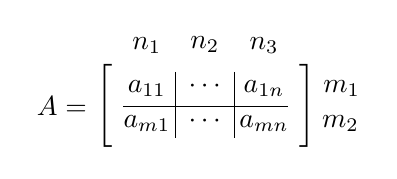
\begin{tikzpicture}[
                every left delimiter/.style={xshift=1ex},
                every right delimiter/.style={xshift=-1ex},
                node distance=1mm
            ]
                \matrix (m) [nodes={minimum width=6mm},matrix of math nodes,left delimiter={[},right delimiter={]}] {
                    a_{11} & \cdots & a_{1n}\\
                    a_{m1} & \cdots & a_{mn}\\
                };
                \draw ([xshift=-3mm]$(m-1-1)!0.5!(m-2-1)$) -- ([xshift=3mm]$(m-1-3)!0.5!(m-2-3)$);
                \draw ([yshift=2mm]$(m-1-1)!0.5!(m-1-2)$) -- ([yshift=-2mm]$(m-2-1)!0.5!(m-2-2)$);
                \draw ([yshift=2mm]$(m-1-2)!0.5!(m-1-3)$) -- ([yshift=-2mm]$(m-2-2)!0.5!(m-2-3)$);
                \node [left=of m] {$A=$};
                \foreach \x in {1,2,3} {
                    \node [above=of m-1-\x] {$n_\x$};
                }
                \node [right=7pt of m-1-3] {$m_1$};
                \node [right=5pt of m-2-3] {$m_2$};
            \end{tikzpicture}
            \caption{Matrix $A$.}
            \label{fig:partitiona}
        \end{subfigure}
        \begin{subfigure}[b]{0.3\linewidth}
            \centering
            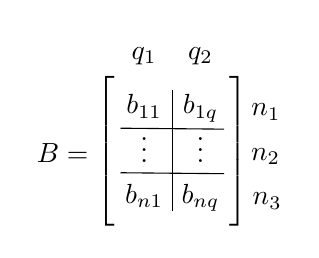
\begin{tikzpicture}[
                every left delimiter/.style={xshift=1ex},
                every right delimiter/.style={xshift=-1ex},
                node distance=1mm,
                every node/.style={text height=.8em}
            ]
                \matrix (m) [nodes={minimum width=6mm},matrix of math nodes,left delimiter={[},right delimiter={]}] {
                    b_{11} & b_{1q}\\
                    \vdots & \vdots\\
                    b_{n1} & b_{nq}\\
                };
                \draw ([xshift=-3mm]$(m-1-1)!0.5!(m-2-1)$) -- ([xshift=3mm]$(m-1-2)!0.5!(m-2-2)$);
                \draw ([xshift=-3mm]$(m-2-1)!0.5!(m-3-1)$) -- ([xshift=3mm]$(m-2-2)!0.5!(m-3-2)$);
                \draw ([yshift=2mm]$(m-1-1)!0.5!(m-1-2)$) -- ([yshift=-2mm]$(m-3-1)!0.5!(m-3-2)$);
                \node [left=of m] {$B=$};
                \foreach \x in {1,2} {
                    \node [above=of m-1-\x] {$q_\x$};
                }
                \node [right=5pt of m-1-2] {$n_1$};
                \node [right=6pt of m-2-2] {$n_2$};
                \node [right=5pt of m-3-2] {$n_3$};
            \end{tikzpicture}
            \caption{Matrix $B$.}
            \label{fig:partitionb}
        \end{subfigure}
        \caption{Partitioning matrices.}
        \label{fig:partition}
    \end{figure}
    \item Each matrix can now be thought of as a matrix of matrices, as follows.
    \renewcommand{\arraystretch}{1.4}
    \begin{align*}
        A &=
        \begin{bmatrix}
            A_{11} & A_{12} & A_{13}\\
            A_{21} & A_{22} & A_{23}\\
        \end{bmatrix}&
        B &=
        \begin{bmatrix}
            B_{11} & B_{12}\\
            B_{21} & B_{22}\\
            B_{31} & B_{32}\\
        \end{bmatrix}
    \end{align*}
    \begin{itemize}
        \item Note that the dimensions of $A_{ij}$ are $m_i\times n_j$ while the dimensions of $B_{ij}$ are $n_i\times q_j$.
        \item Note that the submatrices are composed of the corresponding partitioned values from the matrices in Figure \ref{fig:partition}.
    \end{itemize}
    \item Thus, the product $C=AB$ can be thought of as the following matrix.
    \begin{equation}\label{eqn:partitionmat}
        C = AB =
        \begin{bmatrix}
            C_{11} & C_{12}\\
            C_{21} & C_{22}\\
        \end{bmatrix}
        =
        \begin{bmatrix}
            A_{11}B_{11}+A_{12}B_{21}+A_{13}B_{31} & A_{11}B_{12}+A_{12}B_{22}+A_{13}B_{32}\\
            A_{21}B_{11}+A_{22}B_{21}+A_{23}B_{31} & A_{21}B_{12}+A_{22}B_{22}+A_{23}B_{32}\\
        \end{bmatrix}
    \end{equation}
    \renewcommand{\arraystretch}{1}
    \begin{itemize}
        \item Note that $C_{ij}$ is an $m_i\times q_j$ matrix.
    \end{itemize}
    \item Define the element of $\mathfrak{R}$ at $C_{kl}$ as follows.
    \begin{equation}\label{eqn:partitionsum}
        C_{kl} = \sum_{t=1}^n a_{kt}b_{tl}
        = \sum_{t=1}^{n_1} a_{kt}b_{tl} + \sum_{t=n_1+1}^{n_2} a_{kt}b_{tl} + \sum_{t=n_1+n_2+1}^{n_3} a_{kt}b_{tl}
    \end{equation}
    \item If $1\leq k\leq m_1$ and $1\leq l\leq q_1$, then the three summations on the right of Equation \ref{eqn:partitionsum} are equal to the elements in the $k$-th row and $l$-th column of $A_{11}B_{11}$, $A_{12}B_{21}$, and $A_{13}B_{31}$, respectively.
    \item By Equation \ref{eqn:partitionmat}, the sum of these three elements gives the element in the $k$-th row and $l$-th column of $C_{11}$, which is also the element in the $k$-th row and $l$-th column of $C$.
    \begin{itemize}
        \item This is confirmed by Equation \ref{eqn:partitionsum}.
    \end{itemize}
    \item This process can be continued to confirm the validity of every other submatrix comprising $C$. Therefore, block multiplication is valid.
    \item If two matrices of identical dimensions are partitioned the same way, then block addition and subtraction are valid, too.
\end{itemize}
\newpage



\section{Elementary Properties of Determinants}
\subsection{The Determinant of a Square Matrix}
From \cite{bib:determinants}.
\begin{itemize}
    \item Consider an $n$-square matrix $A$, as below, where all entries are elements of a field $\mathfrak{F}$.
    \begin{equation*}
        A=
        \begin{bmatrix}
            a_{11} & a_{12} & \cdots & a_{1n}\\
            a_{21} & a_{22} & \cdots & a_{2n}\\
            \vdots & \vdots & \ddots & \vdots\\
            a_{n1} & a_{n2} & \cdots & a_{nn}
        \end{bmatrix}
    \end{equation*}
    \item Certain \textbf{scalar functions}, like the \textbf{determinant}, are associated with $A$.
    \item \textbf{Scalar function}: An element of $\mathfrak{F}$ which is of great importance to a matrix.
    \item \textbf{Determinant}: The quantity $|A|\in\mathfrak{F}$ given by Equation \ref{eqn:determinant}, which is the sum of all $n!$ products \dq[ of $A$ and where $\sigma$ is the number of \textbf{negative pairs} among the factors of each product]{that can be obtained by picking one and only one element from each row and from each column}{bib:determinants}{14}
    \begin{equation}\label{eqn:determinant}
        |A| = \sum^{n!}(-1)^\sigma a_{1i_1}\dots a_{ni_n}
    \end{equation}
    \begin{itemize}
        \item Note that $i_1,\dots,i_n$ denotes all $n!$ permutations of the set $\mathbb{Z}\cap[1,n]$.
    \end{itemize}
    \item \textbf{Negative pair}: Two elements $a_{ij}$ and $a_{kl}$ of $A$ such that $i\neq k$ and $j\neq l$ where one of these elements lies to the right of and above the other in $A$.
    \item \textbf{Positive pair}: Two elements $a_{ij}$ and $a_{kl}$ of $A$ such that $i\neq k$ and $j\neq l$ that are not a negative pair.
    \item \textbf{Expansion} (of $|A|$): The unsimplified right side of Equation \ref{eqn:determinant}.
    \item \textbf{Normal} (order): An arbitrary permutation of a set defined to be "standard" for the purpose of finding deviations from this standard.
    \item \textbf{Inversion}: An instance in a permutation of a set where a value \dq{is followed by one which in the normal order proceeds it}{bib:determinants}{15}
    \item The number of inversions in a permutation of $i_1,\dots,i_n$ equals $\sigma$ for the corresponding term in the expansion of $|A|$.
    \begin{itemize}
        \item For two terms $a_{ij}$ and $a_{kl}$, impose the condition that $i<k$.
        \item Thus, whether $j<l$ or $j>l$ determines both whether or not an inversion exists in $i_1,\dots,i_n$ and whether or not $a_{ij}$ and $a_{kl}$ are a positive or a negative pair.
    \end{itemize}
\end{itemize}


\subsection{Elementary Theorems Concerning Determinants}
\begin{itemize}
    \item \textbf{Transpose} (of a matrix): The $n\times m$ matrix $A'$ where the rows of the $m\times n$ matrix $A$ become are the columns of $A'$ without their relative order being altered$^[$\footnote{Transposed matrices are commonly denoted $A^\T$, as in even other parts of this document. Thus, the $A^\T$ notation will continue to be used despite the difference from \cite{bib:determinants}. This definition is the sole exception.}$^]$.
    \begin{itemize}
        \item Denote the element in the $i$-th row and $j$-th column of $A^\T$ as $a^\T_{ij}$.
        \item Thus, $a^\T_{ij}=a_{ji}$.
    \end{itemize}
    \item \textbf{Conjugate} (of a matrix): The matrix $\bar{A}$ obtained by replacing each element $a_{ij}$ of $A$ by it's complex conjugate $\bar{a}_{ij}$.
    \item \textbf{Conjugate transpose} (of a matrix): The matrix $A^*$ that can be thought of either as the transpose of $\bar{A}$ or as the conjugate of $A^\T$.
    \item \newtrm{trm:Tequal}\dq{If $A$ is a square matrix, $|A|=\left|A^\T\right|$}{bib:determinants}{16}
    \begin{itemize}
        \item Each product in Equation \ref{eqn:determinant} has only one element from every row and column of $A$.
        \item Thus, each product in Equation \ref{eqn:determinant} has only one element from every row and column of $A^\T$.
        \item A positive or negative pair of elements in $A$ remains a positive or negative pair under transposition.
        \item Therefore, the terms of Equation \ref{eqn:determinant} are the same for $A$ and $A^\T$.
    \end{itemize}
    \item Note that this theorem implies that for every theorem of determinants concerning the columns of a matrix, there is a corresponding theorem concerning the rows.
    \item \newtrm{trm:BARequal}\dq{If $\Delta=|A|$, then $\bar{\Delta}=|\bar{A}|$}{bib:determinants}{16}
    \begin{itemize}
        \item Follows from the algebraic facts that
        \begin{enumerate}
            \item the conjugate of the sum of two complex numbers equals the sum of the conjugates of said numbers and
            \item the conjugate of the product of two complex numbers equals the product of the conjugates of said numbers.
        \end{enumerate}
        \item Since Equation \ref{eqn:determinant} is a sum of products, the theorem is implied.
    \end{itemize}
    \item \newtrm{trm:row0s}\dq{If all the elements of a row (or of a column) of a square matrix $A$ are zero, then $|A|=0$}{bib:determinants}{16}
    \begin{itemize}
        \item Each product in Equation \ref{eqn:determinant} contains as a factor an element of the row or column of zeros.
        \item Thus, each product equals zero.
        \item Because $\sum 0=0$, $|A|=0$.
    \end{itemize}
    \item \newtrm{trm:kscaled}\dq{If all the elements of a row (or of a column) of a square matrix $A$ be multiplied by an element $k$ of the field, the determinant of the matrix is multiplied by $k$}{bib:determinants}{16} See Equation \ref{eqn:columnk}.
    \begin{equation}\label{eqn:columnk}
        \renewcommand{\arraystretch}{1.4}
        \begin{vmatrix}
            a_1 & b_1 & kc_1\\
            a_2 & b_2 & kc_2\\
            a_3 & b_3 & kc_3\\
        \end{vmatrix}
        = k
        \begin{vmatrix}
            a_1 & b_1 & c_1\\
            a_2 & b_2 & c_2\\
            a_3 & b_3 & c_3\\
        \end{vmatrix}
    \end{equation}
    \begin{itemize}
        \item Each product in Equation \ref{eqn:determinant} contains as a factor an element of the scaled row or column.
        \item Thus, each product is scaled by $k$.
        \item Because $\sum kx=k\sum x$, Equation \ref{eqn:columnk} holds in all instances.
    \end{itemize}
    \item \newtrm{trm:ijswitch}\dq{If two rows (or two columns) of a matrix are interchanged, the determinant of the matrix changes sign}{bib:determinants}{17}
    \begin{itemize}
        \item Let $A_1$ be the matrix identical to $A$ save the row swap.
        \item The language herein will discuss only rows, but the word, "column," could be substituted in every instance.
        \item Case 1: Two adjacent rows are interchanged.
        \begin{itemize}
            \item Clearly, the products are the same in the expansion of both $|A|$ and $|A_1|$.
            \item If a pair of elements contains either zero or only one element in the swapped rows, its identity as a positive or negative pair does not change.
            \item If both elements in a pair are elements of the swapped rows, its identity as a positive or negative pair flips.
            \item Thus, the row swap causes every $\sigma$ to change by $\pm 1$.
        \end{itemize}
        \item Case 2: The $i$-th and $j$-th rows are interchanged where $|i-j|>1$.
        \begin{itemize}
            \item There are $k=|i-j|-1$ rows between the $i$-th and $j$-th rows.
            \item Use $k+1$ adjacent row swaps to move the $j$-th row to the $i$-th position.
            \item Then, use $k$ adjacent row swaps to move the former $i$-th row to the $j$-th position.
            \item Since $2k+1$ row swaps were used, the sign of $|A|$ flipped $2k+1$ times (an odd number of times) during the process.
        \end{itemize}
    \end{itemize}
    \item \newtrm{trm:ident0}\dq{If two rows (or columns) of a matrix $A$ are identical, then $|A|=0$$^[$\footnote{Exception: If the elements of $A$ lie in a field of \textbf{characteristic} 2.}$^]$}{bib:determinants}{17}
    \begin{itemize}
        \item Let $A_1$ be the matrix obtained by swapping the two identical rows.
        \item Since the swapped rows are identical, $A=A_1$.
        \item Thus, $|A|=|A_1|$.
        \item By the previous theorem, $|A_1|=-|A|$, so the following holds.
        \begin{align*}
            |A| &= -|A|\\
            2|A| &= 0\\
            |A| &= 0
        \end{align*}
    \end{itemize}
    \item \newtrm{trm:prop0}\dq{If two rows (or columns) of a matrix $A$ are proportional [dependent], then $|A|=0$}{bib:determinants}{17}
    \begin{itemize}
        \item Let the two proportional rows $R_i$ and $R_j$ be related by $R_j = kR_i$.
        \item Let $A_1$ be the matrix where row $R_j$ is replaced by $R_i$.
        \item By Theorem \ref{trm:kscaled}, $|A|=k|A_1|$.
        \item By Theorem \ref{trm:ident0}, $|A_1|=0$.
        \item Therefore, $|A|=k\times 0=0$.
    \end{itemize}
    \item \textbf{Minor} (of an element $a_{ij}$): The determinant of the $(n-1)$-square matrix resulting from deleting $i$-th row and the $j$-th column of $n$-square matrix $A$.
    \begin{itemize}
        \item Denoted by $|M_{ij}|$.
    \end{itemize}
    \item \textbf{Cofactor} (of an element $a_{ij}$): The signed minor $(-1)^{i+j}|M_{ij}|$.
    \begin{itemize}
        \item Denoted by $\alpha_{ij}$.
    \end{itemize}
    \item \newtrm{trm:cofactor}\dq{The value of the determinant $|A|$ is equal to the sum of the products of the elements of any row (or column) of [$n$-square matrix] $A$, each by its own cofactor}{bib:determinants}{18} See Equation \ref{eqn:cofactor}, where $i,j=1,2,\dots,n$.
    \begin{equation}\label{eqn:cofactor}
        |A| = \sum_{t=1}^na_{it}\alpha_{it} = \sum_{t=1}^na_{tj}\alpha_{tj}
    \end{equation}
    \begin{itemize}
        \item Prove Theorem \ref{trm:cofactor} for row 1:
        \begin{itemize}
            \item The left summation in Equation \ref{eqn:cofactor} can be written as follows. Thus, prove that $k_t=\alpha_{1t}$.
            \begin{equation*}
                |A|=a_{11}k_1+a_{12}k_2+\dots+a_{1n}k_n
            \end{equation*}
            \item The terms in $|A|$ that involve $a_{11}$ are as follows. Note that $a_{11}$ can be moved outside the sum because $a_{11}$ forms a positive pair with every other element and, thus, does not affect $\sigma$.
            \begin{align*}
                \sum (-1)^\sigma a_{11}a_{2i_2}\dots a_{ni_n} &= a_{11}\sum (-1)^\sigma a_{2i_2}a_{3i_3}\dots a_{ni_n}\\
                &= a_{11}|M_{11}|\\
                &= (-1)^{1+1}a_{11}|M_{11}|\\
                &= a_{11}\alpha_{11}
            \end{align*}
            \item For every other element $a_{1t}$, move column $t$ over by $t-1$ columns to place $a_{1t}$ in the $(1,1)$ position.
            \item By the proof of Theorem \ref{trm:ijswitch}, the determinant of the new matrix is $(-1)^{t-1}|A|$.
            \item Note that $M_{1t}$ has not been altered by this process.
            \item Since $a_{1t}|M_{1t}|$ gives all terms involving $a_{1t}$ in the expansion of $(-1)^{t-1}|A|$, multiplying through by $(-1)^{t+1}$ reveals that $a_{1t}\alpha_{1t}$ gives all terms involving $a_{1t}$ in the original determinant $|A|$.
        \end{itemize}
        \item Use the same method$^[$\footnote{Return to this method at a later date. This does not make sense.}$^]$ of moving rows and then multiplying through to prove the general case.
    \end{itemize}
    \item \newtrm{trm:ithsum}\dq{If the $i$-th row of an $n$-square matrix $A$ consists of binomial elements:$$a_{i1}+a'_{i1},a_{i2}+a'_{i2},\dots,a_{in}+a'_{in},$$the determinant $|A|$ is equal to the sum of two determinants, one of which has as its $i$-th row, $a_{i1},a_{i2},\dots,a_{in}$, the other having as its $i$-th row $a'_{i1},a'_{i2},\dots,a'_{in}$, the remaining rows in both determinants being the same as the corresponding rows in the original matrix}{bib:determinants}{19} See Equation \ref{eqn:ithsum}.
    \begin{equation}\label{eqn:ithsum}
        \begin{vmatrix}
            a_{11} & a_{12} & \cdots & a_{1n}\\
            \vdots & \vdots & \cdots & \vdots\\
            a_{i1}+a'_{i1} & a_{i2}+a'_{i2} & \cdots & a_{in}+a'_{in}\\
            \vdots & \vdots & \cdots & \vdots\\
            a_{n1} & a_{n2} & \cdots & a_{nn}\\
        \end{vmatrix}
        =
        \begin{vmatrix}
            a_{11} & a_{12} & \cdots & a_{1n}\\
            \vdots & \vdots & \cdots & \vdots\\
            a_{i1} & a_{i2} & \cdots & a_{in}\\
            \vdots & \vdots & \cdots & \vdots\\
            a_{n1} & a_{n2} & \cdots & a_{nn}\\
        \end{vmatrix}
        +
        \begin{vmatrix}
            a_{11} & a_{12} & \cdots & a_{1n}\\
            \vdots & \vdots & \cdots & \vdots\\
            a'_{i1} & a'_{i2} & \cdots & a'_{in}\\
            \vdots & \vdots & \cdots & \vdots\\
            a_{n1} & a_{n2} & \cdots & a_{nn}\\
        \end{vmatrix}
    \end{equation}
    \begin{itemize}
        \item By Theorem \ref{trm:cofactor}, expand $|A|$ according to the $i$-th row and note that the related cofactors of every matrix in Equation \ref{eqn:ithsum} are identical.
        \begin{equation*}
            \sum_{t=1}^n \left( a_{it}+a'_{it} \right)\alpha_{it} = \sum_{t=1}^n a_{it}\alpha_{it}+\sum_{t=1}^n a'_{it}\alpha_{it}
        \end{equation*}
    \end{itemize}
    \item \newtrm{trm:rowreduction}\dq{If to the elements of any row (or column) of a matrix $A$ we add the products of the corresponding elements of any other row (or column) by the same element $k$ of the field, the determinant of the matrix is unchanged}{bib:determinants}{20}
    \begin{itemize}
        \item Let $A_1$ be identical to matrix $A$ except that every element (scaled by $k$) of $R_i$ is added to the corresponding element of $R_j$.
        \item Let $A_2$ be identical to matrix $A$ except that every element of $R_j$ has been replaced by the corresponding element (scaled by $k$) of $R_i$.
        \item By Theorem \ref{trm:ithsum}, $|A_1|=|A|+|A_2|$.
        \item By Theorem \ref{trm:prop0}, $|A_2|=0$.
        \item Therefore, $|A_1|=|A|+0=|A|$.
    \end{itemize}
    \item \newtrm{trm:ijcofactors0}\dq{The sum of the products of the elements of any row (or column) by the corresponding cofactors of the elements of another row (or column) is zero}{bib:determinants}{20} See Equation \ref{eqn:ijcofactors0}, where $i\neq j$.
    \begin{equation}\label{eqn:ijcofactors0}
        \sum_{t=1}^na_{it}\alpha_{jt}=0
    \end{equation}
    \begin{itemize}
        \item Let $A_1$ be the matrix obtained by replacing the elements of the $j$-th row with the corresponding elements of the $i$-th row.
        \item By Theorem \ref{trm:ident0}, $|A_1|=0$.
        \item The cofactors of the $j$-th row of $A_1$ are identical to those of the $j$-th row of $A$.
        \item The $i$-th row of $A_1$ is identical to that of $A$.
        \item Therefore, the summation in Equation \ref{eqn:ijcofactors0}, which is applicable to both $A_1$ and $A$, equals $|A_1|=0$.
    \end{itemize}
    \item Leopold Kronecker introduced the idea of the \textbf{Kronecker delta}.
    \item \textbf{Kronecker delta}: The symbol $\delta_{ij}$ which stands for 1 if $i=j$ and 0 otherwise.
    \item Using the Kronecker delta, the gist of Theorems \ref{trm:cofactor} and \ref{trm:ijcofactors0} can be combined in the following equation, where $i,j=1,2,\dots,n$.
    \begin{equation*}
        \delta_{ij}|A| = \sum_{t=1}^na_{it}\alpha_{jt} = \sum_{t=1}^na_{ti}\alpha_{tj}
    \end{equation*}
\end{itemize}


\subsection{Laplace's Expansion of a Determinant}
\begin{itemize}
    \item Let $A$ be an $m\times n$ matrix.
    \item \dq{Let $s$ and $t$ be two positive integers such that $s\leq m$ [and] $t\leq n$}{bib:determinants}{21}
    \item \textbf{Minor matrix} (of $A$): The $s\times t$ matrix $A_{j_1,j_2,\dots,j_t}^{i_1,i_2,\dots,i_s}$ that lies in the $i_1,i_2,\dots,i_s$ rows and in the $j_1,j_2,\dots,j_t$ columns of $A$.
    \item \textbf{Minor determinant} (of $A$): The determinant $\left|A_{j_1,j_2,\dots,j_t}^{i_1,i_2,\dots,i_s}\right|$ of a minor matrix of $A$ where $s=t$.
    \item \textbf{Complementary minor} (of a minor matrix): The $(m-s)\times(n-t)$ matrix $A_{j_{t+1},\dots,j_n}^{i_{s+1},\dots,i_m}$ that lies in the $i_{s+1},i_{s+2},\dots,i_m$ rows and in the $j_{t+1},j_{t+2},\dots,j_n$ columns of $A$.
    \begin{itemize}
        \item Note that only a minor matrix with $s<m$ and $t<n$ has a complementary minor.
        \item Note that the matrix $A_{j_1,j_2,\dots,j_t}^{i_1,i_2,\dots,i_s}$ is also the complementary minor of $A_{j_{t+1},\dots,j_n}^{i_{s+1},\dots,i_m}$.
    \end{itemize}
    \item \textbf{Algebraic complement} (of the minor determinant $\left|A_{j_1,\dots,j_s}^{i_1,\dots,i_s}\right|$): The $(n-s)$-rowed signed determinant $(-1)^\rho \left|A_{j_{s+1},\dots,j_n}^{i_{s+1},\dots,i_n}\right|$ where $\rho = i_1+\cdots+i_s+j_1+\cdots+j_s$.
    \begin{itemize}
        \item Note that since $\sigma = i_{s+1}+\cdots+i_n+j_{s+1}+\cdots+j_n$ for the signed determinant, the following proves that $\rho$ and $\sigma$ are either both even or both odd.
        \begin{align*}
            \rho+\sigma &= i_1+\cdots+i_n+j_1+\cdots+j_n\\
            &= 2(1+\cdots+n)
        \end{align*}
    \end{itemize}
    \item \newtrm{trm:algcompment}\dq{If $M=A_{j_1,\dots,j_s}^{i_1,\dots,i_s}$ and $N=A_{j_{s+1},\dots,j_n}^{i_{s+1},\dots,i_n}$ are complementary minor matrices in a square matrix $A$, and if $(-1)^\rho|N|$ is the algebraic complement of $|M|$, then $(-1)^\rho|M|$ is the algebraic complement of $|N|$}{bib:determinants}{21}
    \item \textbf{Principal minor} (matrix): A minor matrix $A_{i_1,i_2,\dots,i_s}^{i_1,i_2,\dots,i_s}$.
    \item \textbf{Principal minor} (determinant): The determinant $\left|A_{i_1,i_2,\dots,i_s}^{i_1,i_2,\dots,i_s}\right|$ of a principal minor matrix.
    \item \dq{The algebraic complement of a principal minor determinant is the same as its plain complement}{bib:determinants}{22}
    \item Consider $A$ to be one of its own minor matrices. In this case, the algebraic complement of $|A|$ is defined as 1.
    \item Theorem \ref{trm:laplace} is known as \textbf{Laplace's Theorem}, as it was discovered by the French mathematician Pierre-Simon Laplace.
    \item \newtrm{trm:laplace}\dq{Let $A$ be an $n$-square matrix with elements in a field $\mathfrak{F}$. From $A$ select any $s$ rows, say the $i_1,i_2,\dots,i_s$ rows. From these $s$ rows form all the $s$-rowed determinants that can be obtained by selecting $s$ columns, say the $j_1,j_2,\dots,j_s$ columns. There will be $\frac{n!}{s!(n-s)!}$ such determinants. The sum of the products of these minor determinants, each by its algebraic complement, is equal to $|A|$, the determinant of $A$}{bib:determinants}{22} See Equation \ref{eqn:laplace}, where \dq[ and where $\rho$ is defined as above]{the summation extends over all the combinations ($j_1,j_2,\dots,j_s$) of the $n$ columns $1,2,\dots,n$ taken $s$ at a time}{bib:determinants}{22}
    \begin{equation}\label{eqn:laplace}
        \sum (-1)^\rho \left| A_{j_1,\dots,j_s}^{i_1,\dots,i_s} \right|\left|A_{j_{s+1},\dots,j_n}^{i_{s+1},\dots,i_n}\right| = |A|
    \end{equation}
    \begin{itemize}
        \item Prove the theorem for the case where the $s$ rows and columns chosen are rows $1,2,\dots,s$ and columns $1,2,\dots,s$.
        \begin{itemize}
            \item Consider the principal minor determinant $\left|A_{1,\dots,s}^{1,\dots,s}\right|$ and its algebraic complement $\left|A_{s+1,\dots,n}^{s+1,\dots,n}\right|$. The terms of the product of the two are in the form given by Equation \ref{eqn:laplace2}.
            \begin{equation}\label{eqn:laplace2}
                (-1)^\sigma a_{1i_1}\cdots a_{si_s}(-1)^\tau a_{s+1j_{s+1}}\cdots a_{nj_n} = (-1)^\sigma\pi_1(-1)^\tau\pi_2
            \end{equation}
            \item Because $a_{1i_1}\cdots a_{si_s}a_{s+1j_{s+1}}\cdots a_{nj_n}$ contains an element from every row and every column of $A$ and because every element of $\pi_1$ forms a positive pair with every element of $\pi_2$, Equation \ref{eqn:laplace2} equals Equation \ref{eqn:laplace3}.
            \begin{equation}\label{eqn:laplace3}
                (-1)^{\sigma+\tau} a_{1j_1}\cdots a_{nj_n}
            \end{equation}
            \item Equation \ref{eqn:laplace3} is a term in the expansion of $|A|$.
            \item Since all of the $s!$ terms of $\left|A_{1,\dots,s}^{1,\dots,s}\right|$ are distinct from all of the $(n-s)!$ terms of $\left|A_{s+1,\dots,n}^{s+1,\dots,n}\right|$, their product gives $s!(n-s)!$ terms of $|A|$.
        \end{itemize}
        \item Extend the theorem to the case where the $s$ rows chosen are rows $1,2,\dots,s$.
        \begin{itemize}
            \item Consider the minor matrix $M=\left|A_{l_1,\dots,l_s}^{1,\dots,s}\right|$.
            \item Shifting the $l_1$-th column $l_1-1$ columns to the left, the $l_2$-th column $l_2-2$ columns to the left, the intervening columns, and finally the $l_s$-th column $l_s-s$ columns to the left, $M$ is brought to the region that the principal minor determinant occupied in the original case.
            \item $M$ and its complement $N$ have not changed, and the determinant of the new matrix is given by Equation \ref{eqn:laplace4}.
            \begin{equation}\label{eqn:laplace4}
                |A_1| = (-1)^{l_1+\cdots+l_s-(1+\cdots+s)}|A|
            \end{equation}
            \item Multiplying through by $(-1)^\rho$ where $\rho=l_1+\cdots+l_s+(1+\cdots+s)$ yields the following change.
            \begin{align*}
                \sum |M|\cdot|N| &= (-1)^{l_1+\cdots+l_s-(1+\cdots+s)}|A|\\
                \sum |M|(-1)^\rho|N| &= (-1)^{l_1+\cdots+l_s+(1+\cdots+s)}(-1)^{l_1+\cdots+l_s-(1+\cdots+s)}|A|\\
                \sum |M|\cdot[\text{alg. comp. of }|M|] &= |A|
            \end{align*}
            \item Since there are ${n\choose s}=\frac{n!}{s!(n-s)!}$ products $|M|\cdot|N|$, each of which yields (by the results of the original case) $s!(n-s)!$ terms in the expansion of $|A|$, this process of using the first $s$ rows and any set of $s$ columns gives all $n!$ distinct terms in the expansion of $|A|$.
        \end{itemize}
        \item Extend the theorem to the general case.
        \begin{itemize}
            \item Select $s$ rows $k_1,\dots,k_s$.
            \item Shift these rows upward to make them the first $s$ rows.
            \item By the previous case, the following holds.
            \begin{align*}
                \sum |M|(-1)^{l_1+\cdots+l_s+(1+\cdots+s)}|N| &= (-1)^{k_1+\cdots+k_s-(1+\cdots+s)}|A|\\
                \sum (-1)^\sigma|M|(-1)^{l_1+\cdots+l_s+(1+\cdots+s)}|N| &= (-1)^{k_1+\cdots+k_s+(1+\cdots+s)}(-1)^{k_1+\cdots+k_s-(1+\cdots+s)}|A|\\
                \sum |M|(-1)^{k_1+\cdots+k_s+l_1+\cdots+l_s}(-1)^{2(1+\cdots+s)}|N| &= |A|\\
                \sum |M|(-1)^{k_1+\cdots+k_s+l_1+\cdots+l_s}|N| &= |A|\\
                \sum |M|(-1)^\rho|N| &= |A|\\
                \sum |M|\cdot[\text{alg. comp. of }|M|] &= |A|
            \end{align*}
        \end{itemize}
    \end{itemize}
\end{itemize}


\subsection{The Determinant of the Product of Two Matrices}
\begin{itemize}
    \item \newtrm{trm:multconditional}\dq{Let $A=(a_{ij})$ be an $m\times n$ matrix and $B=(b_{ij})$ and $n\times m$ matrix so that $P=AB$ is $m$-square. For $m\leq n$, let $A_{i_1,i_2,\dots,i_m}$ denote the $m$-rowed matrix standing in the $i_1,i_2,\dots,i_m$ columns of $A$ and let $B^{j_1,j_2,\dots,j_m}$ denote the $m$-rowed matrix standing in the $j_1,j_2,\dots,j_m$ rows of $B$. Then for $m\leq n$ $|P|=\sum \left| A_{i_1,i_2,\dots,i_m} \right|\left| B^{j_1,j_2,\dots,j_m} \right|$ where the summation extends over all the $n\choose m$ combinations $i_1,i_2,\dots,i_m$ of $n$ things taken $m$ at a time; while, for $m>n$, $|P|=0$}{bib:determinants}{24}
    \begin{itemize}
        \item Prove the theorem for the case where $m\leq n$.
        \begin{itemize}
            \item The determinant $|P|$ can be written as follows, where each of the summation indices $t_1,\dots,t_m$ range over $1,2,\dots,n$.
            \begin{equation*}
                |P| =
                \begin{vmatrix}
                    \sum a_{1t_1}b_{t_11} & \cdots & \sum a_{1t_m}b_{t_mm}\\
                    \vdots & \ddots &\vdots\\
                    \sum a_{mt_1}b_{t_11} & \cdots & \sum a_{mt_m}b_{t_mm}\\
                \end{vmatrix}
            \end{equation*}
            \item Since each column consists of a sum of $n$ elements (and because of Theorem \ref{trm:ithsum}), $|P|$ can be split into the sum of $n^m$ determinants, each of the following form.
            \begin{equation*}
                \begin{vmatrix}
                    a_{1t_1}b_{t_11} & \cdots & a_{1t_m}b_{t_mm}\\
                    \vdots & \ddots & \vdots\\
                    a_{mt_1}b_{t_11} & \cdots & a_{mt_m}b_{t_mm}\\
                \end{vmatrix}
            \end{equation*}
            \item By Theorem \ref{trm:kscaled}, all matching $b$ terms can be factored out of each column, respectively.
            \begin{equation}\label{eqn:multconditional}
                \begin{vmatrix}
                    a_{1t_1} & \cdots & a_{1t_m}\\
                    \vdots & \ddots & \vdots\\
                    a_{mt_1} & \cdots & a_{mt_m}\\
                \end{vmatrix}
                \cdot
                \left( b_{t_11}\cdots b_{t_mm} \right)
            \end{equation}
            \item By Theorem \ref{trm:ident0}, matrices with two or more rows where the indices $t_j$ are equal vanish.
            \item Let $i_1<i_2<\dots<i_m$ be a selection of $m$ of the number $1,2,\dots,n$. Thus, the following holds.
            \begin{equation*}
                \left| A_{i_1,i_2,\dots,i_m} \right| =
                \begin{vmatrix}
                    a_{1i_1} & \cdots & a_{1i_m}\\
                    \vdots & \ddots & \vdots\\
                    a_{mi_1} & \cdots & a_{mi_m}\\
                \end{vmatrix}
            \end{equation*}
            \item Let $t_1,\dots,t_m$ be a permutation of the $i$s and let $\rho$ denote the number of inversions from the normal order. Thus, Equation \ref{eqn:multconditional} can be written as follows.
            \begin{equation}\label{eqn:multconditional2}
                \left| A_{i_1,i_2,\dots,i_m} \right|(-1)^\rho b_{t_11}\cdots b_{t_mm}
            \end{equation}
            \item As $t_1,\dots,t_m$ ranges over all $m!$ permutations of $i_1,\dots,i_m$, the right term in Equation \ref{eqn:multconditional2} becomes $\left| B^{j_1,j_2,\dots,j_m} \right|$. Therefore, Equation \ref{eqn:multconditional} can be rewritten as stated in the theorem.
        \end{itemize}
        \item Prove the theorem for the case where $m>n$.
        \begin{itemize}
            \item Let $A_1$ be matrix $A$ with $m-n$ columns of zeros adjoined.
            \item Let $B_1$ be matrix $B$ with $m-n$ rows of zeros adjoined.
            \item Note that the above adjunctions are legal because they do not change the product $P=AB$.
            \item Each matrix contains only one $m$-rowed determinant, each of which (by Theorem \ref{trm:row0s}) equals 0.
            \item Thus, by the original case, $|P|=|A_1|\cdot|B_1|=0$.
        \end{itemize}
    \end{itemize}
    \item \newtrm{trm:mult}\dq{If $A$ and $B$ are two $n$-square matrices, then $|AB|=|A||B|$}{bib:determinants}{25}
    \begin{itemize}
        \item This follows directly from Theorem \ref{trm:multconditional}.
    \end{itemize}
    \item Let $A$ be an $m\times n$ matrix, let $B$ be an $n\times q$ matrix, and let the $m\times q$ matrix $AB=P$ be their product.
    \item Let $s$ be a positive integer such that $s\leq m$ and $s\leq q$.
    \item Let $P_{j_1,\dots,j_s}^{i_1,\dots,i_s}$ be the $s$-square matrix lying in the $i_1,\dots,i_s$ rows and in the $j_1,\dots,j_s$ columns of $P$.
    \item Let $C$ be the $s\times n$ matrix consisting of the $i_1,\dots,i_s$ rows of $A$ and let $D$ be the $n\times s$ matrix consisting of the $j_1,\dots,j_s$ columns of $B$.
    \item Therefore, the following holds.
    \begin{equation*}
        CD = A_{1,\dots,n}^{i_1,\dots,i_s}B_{j_1,\dots,j_s}^{1,\dots,n} = P_{j_1,\dots,j_s}^{i_1,\dots,i_s}
    \end{equation*}
    \item Applying Theorem \ref{trm:multconditional} to this case yields Theorem \ref{trm:mult-s}.
    \item \newtrm{trm:mult-s}\dq{Let $A$ be an $m\times n$ matrix and $B$ an $n\times q$ matrix, and let $s$ be a positive integer not greater than $m$ or $q$. If $Q$ is the $s$-square minor matrix lying in the $i_1,i_2,\dots,i_s$ rows and in the $j_1,j_2,\dots,j_s$ columns of the product matrix $P=AB$, then $|Q|=0$ if $s>n$; while if $s\leq n$, $|Q|$ is equal to the sum of $n\choose s$ terms, each term being the product of an $s$-rowed minor determinant lying in the $i_1,i_2,\dots,i_s$ rows and in the $t_1,t_2,\dots,t_s$ colummns of $A$ by an $s$-rowed minor determinant lying in the $t_1,t_2,\dots,t_s$ rows and in the $j_1,j_2,\dots,j_s$ columns of $B$, as $t_1,t_2,\dots,t_s$ runs through all the $n\choose s$ combinations of the $n$ numbers $1,2,\dots,n$ taken $s$ at a time}{bib:determinants}{26} See Equation \ref{eqn:mult-s}.
    \begin{equation}\label{eqn:mult-s}
        |Q| = \left| P_{j_1,\dots,j_s}^{i_1,\dots,i_s} \right| = \sum_t \left| A_{t_1,\dots,t_s}^{i_1,\dots,i_s} \right|\left| B_{j_1,\dots,j_s}^{t_1,\dots,t_s} \right|
    \end{equation}
\end{itemize}
\newpage



\section{Eigenvalues, Eigenvectors, and Invariant Subspaces}
\subsection{Invariant Subspaces}
\begin{itemize}
    \item \textbf{Operator}: A linear map from a vector space to itself.
    \begin{itemize}
        \item Denote the set of operators on a vector space $V$ by $\Li(V)$.
        \item Denote the set of all linear maps from $V$ to $W$ by $\Li(V,W)$ \cite[52]{bib:Axler}.
        \item Denote an operator/element of $\Li(V)$/linear map by $T$.
    \end{itemize}
    \item Let $T$ be an operator on a vector space $V$ that is decomposable into a direct sum of proper subspaces as follows.
    \begin{equation*}
        V = U_1 \oplus\cdots\oplus U_m
    \end{equation*}
    \begin{itemize}
        \item To understand $T$, try to understand each $T|_{U_j}$.
        \begin{itemize}
            \item Let $T|_{U_j}$ denote \dq{the restriction of $T$ to the smaller domain $U_j$}{bib:Axler}{132}
        \end{itemize}
        \item Since $T|_{U_j}$ may not map $U_j$ onto itself in every case, consider only direct sum decompositions $T$ maps each $U_j$ into itself. A subspace that gets mapped onto itself is called an \textbf{invariant subspace}.
    \end{itemize}
    \item \textbf{Invariant subspace} (under $T$): A subspace $U$ of $V$ such that $u\in U \Rightarrow Tu\in U$, where $T\in\Li(V)$.
    \item These subspaces of $V$ are invariant under $T\in\Li(V)$: $\{0\}$, $V$, $\text{null }T$, and $\text{range }T$$^[$\footnote{Note that $\text{range }T$ is equivalent to the column space of $T$, $C(T)$.}$^]$.
    \item Example of an invariant subspace of $V$ besides $\{0\}$ and $V$: \dq{Suppose that $T\in\Li(\mathcal{P}(\R))$ is defined by $Tp=p'$. Then $\mathcal{P}_4(\R)$, which is a subspace of $\mathcal{P}(\R)$, is invariant under $T$ because if $p\in\mathcal{P}(R)$ has degree at most 4, then $p'$ also has degree at most 4}{bib:Axler}{133}
    \begin{itemize}
        \item \textbf{Polynomial}: \dq{A function $p:\F\rightarrow\F$\dots with coefficients in $\F$ [such that] there exist $a_0,\dots,a_m\in\F$ such that$$p(z) = a_0+a_1z+a_2z^2+\cdots+a_mz^m$$for all $z\in\F$}{bib:Axler}{30}
        \item \dq{$\mathcal{P}(\F)$ is the set of all polynomials with coefficients in $\F$}{bib:Axler}{30}
        \item \dq{For $m$ a nonnegative integer, $\mathcal{P}_m(\F)$ denotes the set of all polynomials with coefficients in $\F$ and degree at most $m$}{bib:Axler}{31}
    \end{itemize}
    \item To begin a study of invariant subspaces, consider the simplest possible type of invariant subspace: those for which $\dim U = 1$.
    \item For any $v\in V$ where $v\neq 0$, define $U$ as follows.
    \begin{equation*}
        U = \left\{ \lambda v:\lambda\in\F\right\} = \text{span}(v)
    \end{equation*}
    \item If $U$ is invariant under $T\in\Li(V)$, then $Tv\in U$.
    \item If $Tv\in U$, then there exists $\lambda\in\F$ such that
    \begin{equation}\label{eqn:eigendef}
        Tv = \lambda v
    \end{equation}
    \item \textbf{Eigenvalue} (of $T$): A scalar $\lambda\in\F$ such that there exists $v\in V$ where $v\neq 0$ and Equation \ref{eqn:eigendef} is satisfied. \emph{Also known as} \textbf{characteristic value}$^[$\footnote{"Eigen" is German for "own."}$^]$.
    \item \dq{$T$ has a 1-dimensional invariant subspace if and only if $T$ has an eigenvalue}{bib:Axler}{134}
    \item $\lambda$ is an eigenvalue of $T$, $T-\lambda I$ is not \textbf{injective}, $T-\lambda I$ is not \textbf{surjective}, and $T-\lambda I$ is not invertible are all equivalent conditions that $\lambda\in\F$ must pass to be an eigenvalue of $T\in\Li(V)$, where $V$ is finite dimensional.
    \begin{itemize}
        \item The first and second conditions are equivalent because for $\lambda$ to be an eigenvalue of $T$, Equation \ref{eqn:eigendef} must be satisfied. However, $Tv=\lambda v \Rightarrow (T-\lambda I)v=0$. Furthermore, if $T-\lambda I$ is injective, $N(T-\lambda I)=\{0\}$. But since $v\neq 0$, $T-\lambda I$ cannot be injective.
        \begin{itemize}
            \item From pg. 61: Suppose there exists $v\in\text{null }T$ and $v\neq 0$. Then $Tv=0=T(0)$. But since $T$ is injective, $v=0$, and we have arrived at a contradiction. Therefore, if $T$ is injective, $\text{null }T=\{0\}$.
        \end{itemize}
        \item Invertibility, injectivity, and surjectivity are all equivalent via the fundamental theorem of linear algebra.
    \end{itemize}
    \item \textbf{Injective} (function $T$): A function $T:V\rightarrow W$ such that $Tu=Tv\Rightarrow u=v$. \emph{Also known as} \textbf{one-to-one}.
    \begin{itemize}
        \item \dq{$T$ is injective if it maps distinct inputs to distinct outputs}{bib:Axler}{60}
    \end{itemize}
    \item \textbf{Surjective} (function $T$): A function $T:V\rightarrow W$ such that $\text{range }T=W$.
    \begin{itemize}
        \item The differentiation map $S\in\Li(\mathcal{P}_5(\R),\mathcal{P}_4(\R))$ defined by $Sp = p'$ is surjective because \dq{its range equals $\mathcal{P}_4(\R)$, which is now the vector space into which $S$ maps}{bib:Axler}{62}
    \end{itemize}
    \item \textbf{Eigenvector} (of $T$): A vector $v\in V$, where $v\neq 0$, corresponding to $\lambda\in\F$ that satisfies Equation \ref{eqn:eigendef} for some $T\in\Li(V)$.
    \item \dq{A vector $v\in V$ with $v\neq 0$ is an eigenvector of $T$ corresponding to $\lambda$ if and only if $v\in\text{null}(T-\lambda I)$}{bib:Axler}{135}
    \item Example: Let $T\in\Li(\F^2)$ be defined by $T(w,z)=(-z,w)$.
    \begin{itemize}
        \item Find the eigenvalues and eigenvectors of $T$ if $\F=\R$.
        \begin{figure}[h!]
            \centering
            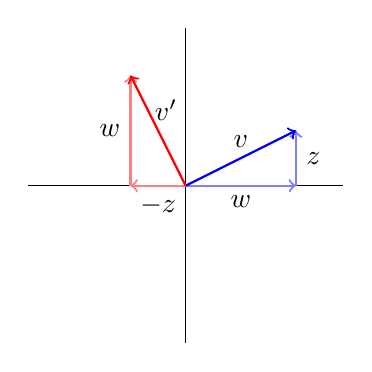
\begin{tikzpicture}[
                vector/.style={color=#1,thick,->,scale=0.7},
                every node/.style={black}
            ]
                \draw (-2,0) -- (2,0);
                \draw (0,-2) -- (0,2);

                \draw [vector=blue!50] (0,0) -- node[below]{$w$} (2,0);
                \draw [vector=blue!50] (2,0) -- node[right]{$z$} (2,1);
                \draw [vector=blue] (0,0) -- node[above]{$v$} (2,1);

                \draw [vector=red!50] (0,0) -- node[below]{$-z$} (-1,0);
                \draw [vector=red!50] (-1,0) -- node[left]{$w$} (-1,2);
                \draw [vector=red] (0,0) -- node[above,xshift=1mm]{$v'$} (-1,2);
            \end{tikzpicture}
            \caption{$T$ provides a $90^\circ$ counterclockwise rotation in $\R^2$.}
            \label{fig:T90counter}
        \end{figure}
        \begin{itemize}
            \item Following from its definition, $T$ provides a counterclockwise rotation of $90^\circ$ in $\R^2$ (see Figure \ref{fig:T90counter}).
            \item Since $T$ can only rotate real vectors (not scale them), it has no eigenvalues or eigenvectors when $\F=\R$.
        \end{itemize}
        \item Find the eigenvalues and eigenvectors of $T$ if $\F=\C$.
        \begin{itemize}
            \item In this case, the left and middle parts of the following equation are equal because of the definition of $T$. Furthermore, the left and right parts must be equal for some $\lambda\in\F$ there are to be eigenvalues.
            \begin{equation*}
                T
                \begin{bmatrix}
                    a+bi\\
                    c+di\\
                \end{bmatrix}
                =
                \begin{bmatrix}
                    -c-di\\
                    a+bi\\
                \end{bmatrix}
                =\lambda
                \begin{bmatrix}
                    a+bi\\
                    c+di\\
                \end{bmatrix}
            \end{equation*}
            \item Focusing on the middle and right parts, separate the vectors into a system of equations, as follows.
            \begin{align*}
                -c-di &= \lambda(a+bi)\\
                a+bi &= \lambda(c+di)
            \end{align*}
            \item Treating the complex numbers $a+bi$ and $c+di$ as single variables, it becomes clear that this system can easily be solved for $\lambda$ by substituting the definition of $a+bi$ given by the second equation, above, into the first equation, above, and simplifying.
            \begin{align*}
                -c-di &= \lambda(\lambda(c+di))\\
                -(c+di) &= \lambda^2(c+di)\\
                -1 &= \lambda^2
            \end{align*}
            \begin{align*}
                \lambda_1 &= i & \lambda_2 &= -i
            \end{align*}
            \item $\lambda_1$ and $\lambda_2$, above, are the eigenvalues of $T$.
            \item Now for the eigenvectors. Returning to the initial vector equation and arbitrarily focusing on $\lambda_1$, consider the following.
            \begin{align*}
                -c-di &= i(a+bi)\\
                -c-di &= ia+i^2b\\
                -c-di &= -b+ai
            \end{align*}
            \item Draw associations between like parts to find $c$ and $d$ in terms of $a$ and $b$.
            \begin{align*}
                -c &= -b & -di &= ai\\
                c &= b & d &= -a
            \end{align*}
            \item Make the above substitutions into the general vector $
                \begin{bmatrix}
                    a+bi\\
                    c+di\\
                \end{bmatrix}
            $ to find the first eigenvector, $x_1$.
            \begin{equation*}
                x_1 =
                \begin{bmatrix}
                    a+bi\\
                    b-ai\\
                \end{bmatrix}
                ,\ a,b\in\R
            \end{equation*}
            \item Repeat the process with $\lambda_2$ to find $x_2$.
            \begin{equation*}
                x_2 =
                \begin{bmatrix}
                    a+bi\\
                    -b+ai\\
                \end{bmatrix}
                ,\ a,b\in\R
            \end{equation*}
            \item Thus, we have two distinct eigenvalues for $T$ and two distinct classes of eigenvectors. Any values of $a$ and $b$ in the forms given for $x_1$ and $x_2$ will be an eigenvector.
        \end{itemize}
    \end{itemize}
    \item Linear independence of eigenvectors: \dq{Let $T\in\Li(V)$. Suppose $\lambda_1,\dots,\lambda_m$ are distinct eigenvalues of $T$ and $v_1,\dots,v_m$ are corresponding eigenvectors. Then $v_1,\dots,v_m$ is linearly independent}{bib:Axler}{136}
    \begin{itemize}
        \item Suppose $v_1,\dots,v_m$ is linearly dependent.
        \begin{itemize}
            \item $\lambda_1,\dots,\lambda_m$ remain distinct.
        \end{itemize}
        \item Let $k$ be the smallest positive integer satisfying the \textbf{Linear Dependence Lemma}.
        \item By said lemma, there exists $a_1,\dots,a_{k-1}\in\F$ such that the following holds.
        \begin{equation*}
            v_k = a_1v_1+\cdots+a_{k-1}v_{k-1}
        \end{equation*}
        \item Apply $T$ to both sides of the above equation to yield the following.
        \begin{equation*}
            \lambda_kv_k = a_1\lambda_1v_1+\cdots+a_{k-1}\lambda_{k-1}v_{k-1}
        \end{equation*}
        \item Subtract the second equation from $\lambda_k$ times the first equation to yield the following.
        \begin{equation*}
            0 = a_1(\lambda_k-\lambda_1)v_1+\cdots+a_{k-1}(\lambda_k-\lambda_{k-1})v_{k-1}
        \end{equation*}
        \item By the criteria under which $k$ was selected, $v_1,\dots,v_{k-1}$ are linearly independent. Thus, for their sum to be 0, all coefficients must equal 0.
        \item By the zero product property, either $a_j$ or $\lambda_k-\lambda_j$, where $j\in\{1,2,\dots,k-1\}$, must equal zero. Since all eigenvalues are distinct, no difference of eigenvalues is 0. Thus, ever $a_j=0$.
        \item However, if $a_j=0$, by the first equation above, $v_k=0$.
        \item Therefore, we have arrived at a contradiction.
    \end{itemize}
    \item \textbf{Linear Dependence Lemma}: If $v_1,\dots,v_m$ is a linearly dependent list in $V$, then there exists at least one value $j\in\{1,2,\dots,m\}$ such that $v_j\in\text{span}(v_1,\dots,v_{j-1})$ and if the $j^\text{th}$ term is removed from $v_1,\dots,v_m$, the span of the remaining list equals $\text{span}(v_1,\dots,v_m)$ \cite[34]{bib:Axler}.
    \item A bound on the number of eigenvalues: \dq{Suppose $V$ is finite-dimensional. Then each operator on $V$ has at most $\dim V$ distinct eigenvalues}{bib:Axler}{136}
    \begin{itemize}
        \item Approach: Prove a bound on the number of eigenvectors.
        \item Let $T\in\Li(V)$ have eigenvalues $\lambda_1,\dots,\lambda_m$.
        \item Thus, $T$ has $m$ linearly independent corresponding eigenvectors $v_1,\dots,v_m$.
        \item Since $\dim(\text{span}(v_1,\dots,v_m))$ cannot exceed $\dim V$, $m\leq\dim V$.
    \end{itemize}
    \item On quotient spaces:
    \begin{itemize}
        \item Let $v+U$ be a subset (not a subspace) of $V$ defined by
        \begin{equation*}
            v+U = \left\{ v+u:v\in V,u\in u \right\}
        \end{equation*}
        \item Example:
        \begin{figure}[h!]
            \centering
            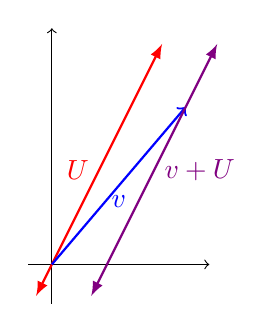
\begin{tikzpicture}
                \draw [->] (-0.3,0) -- (2,0);
                \draw [->] (0,-0.5) -- (0,3);

                \draw [red,thick,latex-latex] (-0.2,-0.4) -- node[anchor=east]{$U$} (1.4,2.8);
                \draw [blue,thick,->] (0,0) -- node[anchor=north]{$v$} (1.7,2);
                \draw [red!50!blue,thick,latex-latex] (0.5,-0.4) -- node[anchor=west]{$v+U$} (2.1,2.8);
            \end{tikzpicture}
            \caption{Visualizing $v+U$.}
            \label{fig:vU}
        \end{figure}
        \begin{itemize}
            \item Let $U=\left\{ (x,2x)\in\R^2:x\in\R \right\}$. Then $U$ can be conceived as the red line (with slope 2) in Figure \ref{fig:vU}.
            \item Let $v\in\R^2$ be $v=(17,20)$ (the blue vector in Figure \ref{fig:vU}).
            \item Then $v+U$ is the subset of $\R^2$ where every vector $u\in U$ has had $v$ added to it. This has the effect of creating a subset $v+U$ (the purple line in Figure \ref{fig:vU}).
        \end{itemize}
        \item \textbf{Affine subset} (of $V$): \dq{A subset of $V$ of the form $v+U$ for some $v\in V$ and some subspace $U$ of $V$}{bib:Axler}{94}
        \item Affine subsets $v+U$ are \textbf{parallel} to $U$.
        \begin{itemize}
            \item See how the purple and red lines are parallel in Figure \ref{fig:vU}.
        \end{itemize}
        \item Note that parallel affine subsets of the $xy$-plane in $\R^3$ are also planes (not lines).
        \item \textbf{Quotient space}: \dq{The set of all affine subsets of $V$ parallel to $U$}{bib:Axler}{95} \emph{Also known as} \textbf{\emph{V}/\emph{U}}. \emph{Symbolically defined as}
        \begin{equation*}
            V/U = \left\{ v+U:v\in V \right\}
        \end{equation*}
    \end{itemize}
    \item \textbf{Restriction operator}: $T|_U(u)\in\Li(U)$ is defined by $T|_U(u)=Tu$ for $u\in U$.
    \begin{itemize}
        \item The fact that $U$ is invariant under $T$ is what allows us to consider $T|_U$ to be in $\Li(U)$ as opposed to just $\Li(V)$.
    \end{itemize}
    \item \textbf{Quotient operator}: $T/U\in\Li(V/U)$ is defined by $(T/U)(v+U)=Tv+U$ for $v\in V$.
    \begin{itemize}
        \item Verify that if $v+U=w+U$, then $Tv+U = Tw+U$.
        \item If $v+U=w+U$, then $v-w\in U\Rightarrow T(v-w)\in U\Rightarrow Tv-Tw\in U\Rightarrow Tv+U=Tw+U$.
    \end{itemize}
    \item $T|_U$ and $T/U$ can tell us about $T$.
    \item However, they also sometimes fail to tell us about $T$:
    \begin{itemize}
        \item Let $T\in\Li(\F^2)$ be defined by $T(x,y)=(y,0)$ and let $U=\left\{ (x,0):x\in\F \right\}$. Show that\dots
        \begin{itemize}
            \item $U$ is invariant under $T$ and $T|_U$ is the 0 operator on $U$.
            \item There does not exist a subspace $W$ of $\F^2$ that is invariant under $T$ and such that $\F^2=U\oplus W$.
            \item $T/U$ is the 0 operator on $\F^2/U$.
        \end{itemize}
        \item First:
        \begin{itemize}
            \item $u=(x,0) \Rightarrow Tu=(0,0)$.
            \item $x\in\F \Rightarrow (0,0)\in U$.
            \item Since every $Tu$ maps $u$ to a value in $U$, $U$ is invariant under $T$. Since that value $Tu$ is 0, $T|_U$ is the 0 operator.
        \end{itemize}
        \item Second:
        \begin{itemize}
            \item $\F^2=U\oplus W \Rightarrow W=\left\{ (0,y):y\in\F \right\}$.
            \item For $w\in W$, $Tw=(y,0)$.
            \item For every $w$ except 0, $T$ maps $w$ into $U$.
        \end{itemize}
        \item Third:
        \begin{align*}
            (T/U)((x,y)+U) &= (T/U)(x,y)+U\\
            &= (y,0)+U\\
            &= U
        \end{align*}
        \begin{itemize}
            \item The last equality holds because $(y,0)\in U$.
            \item Note that $U$ is the 0 of $\F^2/U$.
        \end{itemize}
    \end{itemize}
\end{itemize}
\newpage



\bibliography{GIEPNotes}
\bibliographystyle{apalike}




\end{document}